\documentclass{fefu_presentation}

\usepackage{nicefrac}
\usepackage{graphicx}
\usepackage{multicol}
\usepackage{subcaption}
\usepackage{array}
\usepackage{calc}
\usepackage{xcolor}
\usepackage{tikz}
\usetikzlibrary{positioning,decorations,calc}
\graphicspath{{../images/}}

\newcolumntype{C}[1]{>{\centering\arraybackslash}m{#1}}
\definecolor{redish}{rgb}{0.8,0.2,0.2}
\definecolor{greenish}{rgb}{0,0.7,0.3}

\newif\ifstartcompletesineup
\newif\ifendcompletesineup
\pgfkeys{
    /pgf/decoration/.cd,
    start up/.is if=startcompletesineup,
    start up=true,
    start up/.default=true,
    start down/.style={/pgf/decoration/start up=false},
    end up/.is if=endcompletesineup,
    end up=true,
    end up/.default=true,
    end down/.style={/pgf/decoration/end up=false}
}
\pgfdeclaredecoration{complete sines}{initial}
{
    \state{initial}[
    width=+0pt,
    next state=upsine,
    persistent precomputation={
        \ifstartcompletesineup
        \pgfkeys{/pgf/decoration automaton/next state=upsine}
        \ifendcompletesineup
        \pgfmathsetmacro\matchinglength{
            0.5*\pgfdecoratedinputsegmentlength / (ceil(0.5* \pgfdecoratedinputsegmentlength / \pgfdecorationsegmentlength) )
        }
        \else
        \pgfmathsetmacro\matchinglength{
            0.5 * \pgfdecoratedinputsegmentlength / (ceil(0.5 * \pgfdecoratedinputsegmentlength / \pgfdecorationsegmentlength ) - 0.499)
        }
        \fi
        \else
        \pgfkeys{/pgf/decoration automaton/next state=downsine}
        \ifendcompletesineup
        \pgfmathsetmacro\matchinglength{
            0.5* \pgfdecoratedinputsegmentlength / (ceil(0.5 * \pgfdecoratedinputsegmentlength / \pgfdecorationsegmentlength ) - 0.4999)
        }
        \else
        \pgfmathsetmacro\matchinglength{
            0.5 * \pgfdecoratedinputsegmentlength / (ceil(0.5 * \pgfdecoratedinputsegmentlength / \pgfdecorationsegmentlength ) )
        }
        \fi
        \fi
        \setlength{\pgfdecorationsegmentlength}{\matchinglength pt}
    }] {}
    \state{downsine}[width=\pgfdecorationsegmentlength,next state=upsine]{
        \pgfpathsine{\pgfpoint{0.5\pgfdecorationsegmentlength}{0.5\pgfdecorationsegmentamplitude}}
        \pgfpathcosine{\pgfpoint{0.5\pgfdecorationsegmentlength}{-0.5\pgfdecorationsegmentamplitude}}
    }
    \state{upsine}[width=\pgfdecorationsegmentlength,next state=downsine]{
        \pgfpathsine{\pgfpoint{0.5\pgfdecorationsegmentlength}{-0.5\pgfdecorationsegmentamplitude}}
        \pgfpathcosine{\pgfpoint{0.5\pgfdecorationsegmentlength}{0.5\pgfdecorationsegmentamplitude}}
    }
    \state{final}{}
}

\tikzset{
    between/.style args={#1 and #2}{
        at = ($(#1)!0.5!(#2)$)
    }
}

\tikzset{
    between base/.style args={#1 and #2}{
        between=#1.base and #2.base
    }
}

\enablenotes

\newif\ifmetropolis
\metropolistrue

\setgroup{М9119-09.04.01иибд}
\setsupervisor{Петров Павел Сергеевич}{кандидат физико-математических наук\\зав. лаб. 3/2 ТОИ ДВО РАН}
\setschool{цифровой экономики}

\author{Тыщенко Андрей Геннадьевич}
\title[Моделирование звукового поля]{Комплекс программ для моделирования трёхмерных звуковых полей в сложных неоднородных океанических волноводах}
\date{07 июля 2021 г.}

\newif\ifPS
%\PStrue

\ifmetropolis
    \usetheme[progressbar=frametitle,numbering=fraction]{metropolis}
    \makeatletter
    \setlength{\metropolis@progressinheadfoot@linewidth}{2pt}
    \makeatother
\else
    \usetheme{CambridgeUS}
\fi

\setbeamersize{text margin left=3.5mm,text margin right=3.5mm} 

\newcommand{\pa}[1]{\left(#1\right)}

\usepackage{alphalph}
\makeatletter
\newcommand{\makeAlph}[1]{(\alphalph{\arabic{#1}})}
\makeatother

\newcommand*\rot{\rotatebox{90}}
%\newcolumntype{C}[1]{>{\centering\arraybackslash}m{#1}}

\begin{document}
    
    \presentationtitlepage
    
     \note{Защищается студент группы М9119-09.04.01иибд Тыщенко Андрей Геннадьевич по теме Комплекс программ для моделирования трёхмерных звуковых полей в сложных неоднородных океанических волноводах. Руководитель кандидат физико-математических наук, заведующий лабораторией 3/2 ТОИ ДВО РАН Петров Павел Сергеевич.}
    
     \begin{frame}[fragile]{Области применения моделирования звука}
     	\begin{block}{}
             \vspace{-0.5cm}
     		\begin{itemize}
     			\item Оценка уровня антропогенных акустических шумов при выполнении сейсморазведочных работ на восточном шельфе о. Сахалин с целью защиты морских млекопитающих (в т.ч. краснокнижных серых китов)
     			\item Определение зон акустической тени при выборе мест расположения источников навигационных сигналов
     		\end{itemize}
     	\end{block}
         \begin{figure}[h]
             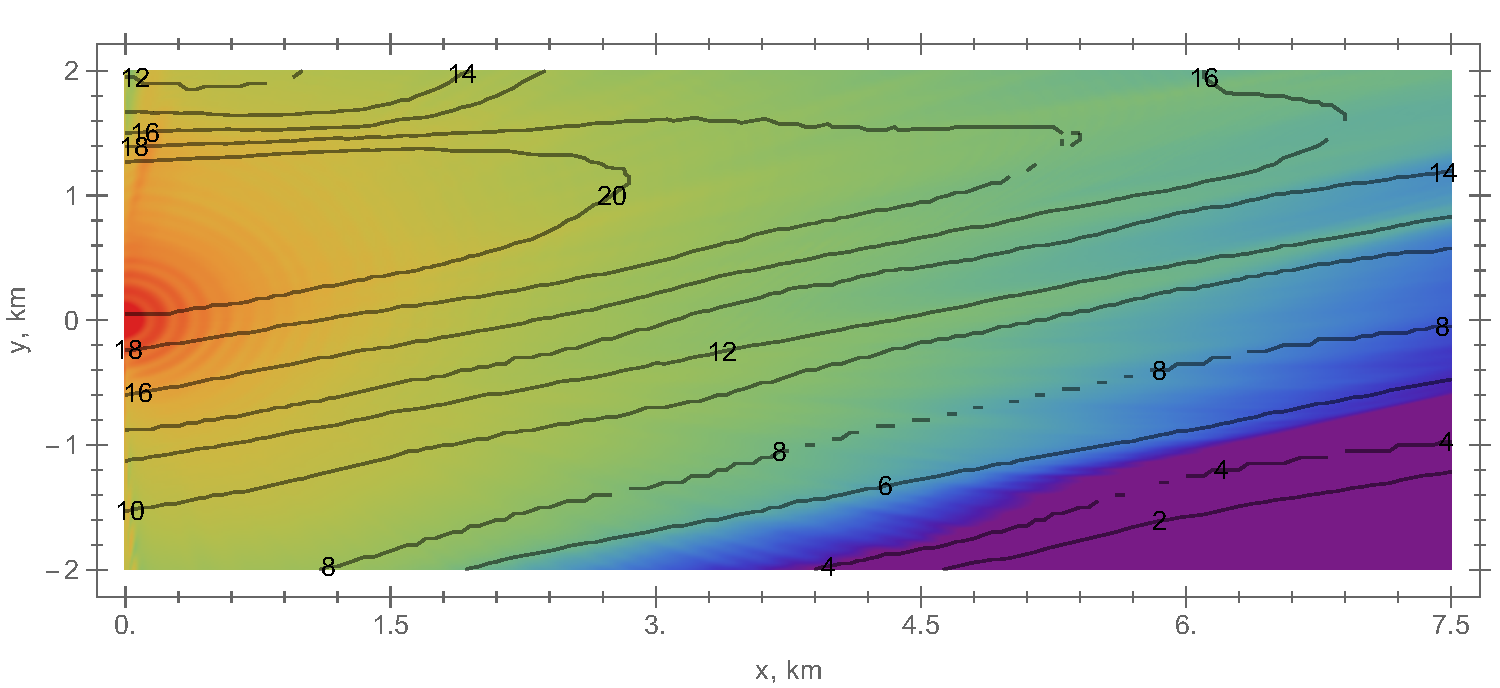
\includegraphics[width=0.7\textwidth]{sel.pdf}
             \caption{Оценка уровня антропогенного шума}
         \end{figure}
     \end{frame}

 	\note{Моделирование трёхмерных звуковых полей применяется во многих областях исследования и освоения океана, например оценка влияния человека на морскую фауну и системы акустической навигации связи. При решении первой задачи необходимо оценить влияние источников звука на морскую фауну. При разработке систем подводной навигации важно знать зоны уверенного сигнала и зоны тени.}
    
     \begin{frame}[fragile]{Цель работы}
     	\begin{block}{}
             Разработка комплекса программ для решения следующих задач
             \begin{itemize}
                 \item Моделирование трёхмерного звукового поля с использованием модового разложения звука
                 \item Трассировка лучей, соответствующих вертикальным модам
                 \item Вычисление временного ряда импульса звукового сигнала в произвольных точках волновода с указанием опорного сигнала в одной из них или функции источника
                 \item Расчёт интегральных характеристик (SEL)
             \end{itemize}
     	\end{block}
         \begin{block}{Методы}
             \begin{itemize}
                 \item Split-step Pad\`e метод решения уравнения горизонтальной рефракции
                 \item Аппроксимация Паде произвольного порядка
             \end{itemize}
         \end{block}
     \end{frame}

 	\note{Целью работы является разработка комплекса программ для моделирования трёхмерного звукового поля с использованием модового разложения звука, предоставляющего возможность расчёта временного ряда импульса звукового сигнала и интегральных характеристик звукового сигнала c применением Split-step Pade метода решения уравнения горизонтальной рефракции и аппроксимации Паде произвольного порядка}
    
     \begin{frame}[fragile]{Звуковое поле}
         \begin{block}{Уравнение Гельмгольца}
             \ifmetropolis
                 \smallskip
             \fi
             \begin{equation}\label{eq::3DH}
                 \pa{\rho\pa{z}\nabla\cdot\pa{\frac{1}{\rho\pa{z}}\nabla} +  K^2\pa{x,y,z}}p\pa{x,y,z}=-\delta\pa{x}\delta\pa{y}\delta\pa{z-z_s}
             \end{equation}
             \begin{equation*}
                 K\pa{z}=\frac{\omega}{c\pa{z}}\pa{1+i\eta\beta}
             \end{equation*}
             \centering
             \begin{tabular}{ll}
                  $\rho\pa{z}$ --- плотность среды & $c\pa{z}$ --- скорость звука\\
                  $\omega=2\pi f$ --- циклическая частота & $\beta$ --- коэффициент затухания\\
                  $\eta=\nicefrac{1}{40\pi\log_{10}e}$&
             \end{tabular}
         \end{block}
     \end{frame}

 	\note{Звуковое поле, создаваемое точечным источником в трёхмерном волноводе мелкого моря, описывается трёхмерным уравнением Гельмгольца. Здесь $x,y$ --- горизонтальные координаты, $z$ --- глубина (положительная величина), $\rho\pa{z}$ --- плотность. Может быть рассмотрено два случая: с учётом затухания волн и без, зависящее от значения коэффициента затухания $\beta$. Здесь $c\pa{z}$ --- скорость звука на глубине $z$. $\omega$ --- циклическая частота ($f$ -- частота источника), $\eta$ --- вот такое странное число.}

     \begin{frame}[fragile]{Модовое разложение поля}
         \begin{block}{Модовое разложение}
             \ifmetropolis
                 \smallskip
             \fi
             \begin{equation}
                 p\pa{x,y,z}=\sum\limits_{j=1}^JA_j\pa{x,y}\varphi_j\pa{z,x,y}
             \end{equation}
         \end{block}
         \begin{block}{Уравнение горизонтальной рефракции}
             \ifmetropolis
                 \smallskip
             \fi
             \begin{equation}
                 \frac{\partial^2 A_j}{\partial x^2} + \frac{\partial^2 A_j}{\partial y^2}+k_j^2 (x,y)A_j=-\varphi_j(z_s)\delta(x)\delta(y)
             \end{equation}
         \end{block}
         \begin{block}{Псевдодифференциальное МПУ}
             \ifmetropolis
                 \smallskip
             \fi
             \begin{equation}
                 A_j\pa{x,y}=e^{k_{j,0}x}\mathcal{A}_j\pa{x,y}
             \end{equation}
             \begin{equation}
                 \frac{\partial\mathcal{A}_j\pa{x,y}}{\partial x}=ik_{j,0}\pa{\sqrt{1+L_j}-1}\mathcal{A}_j\pa{x,y}
             \end{equation}
             \begin{equation}
                 k_{j,0}^2L_j=\frac{\partial^2}{\partial y^2}+k_j^2\pa{x,y}-k_{j,0}^2\nonumber
             \end{equation}
         \end{block}
     \end{frame}

 	\note{Решение $p\pa{x,y,z}$ уравнения Гельмгольца может быть выражено в форме модового разложения, где $A_j$ --- модовые амплитуды, а $\varphi_j$ ---модовые функции. Модовые аплитуды удовлетворяют уравнению горизонтальной рефракции, где $z_s$ --- глубина источника. Модовые функции $\varphi_j\pa{z,x,y}$ и соответствующие им горизонтальные числа $k_j(x,y)$ могут быть получены из решения акустической спектральной задачи. Таким образом появляется возможность рассматривать уравнение для каждой моды отдельно. Учитывая звуковые волны, распространяющиеся в положительном направлении оси $x$ и вводя относительное волновое число $k_{j,0}$ получим псевдо-дифференциальное модовое параболическое уравнение.}

     \begin{frame}[fragile]{Аппроксимация оператора квадратного корня}
         \begin{block}{Аппроксимация Паде для функции $F\pa{\lambda}$}
             \ifmetropolis
                 \smallskip
             \fi
             \begin{equation}
                 F\pa{\lambda}\approx\mathcal{R}\pa{F,l,m}\pa{\lambda}\equiv\frac{P^F_{l,m}\pa{\lambda}}{Q^F_{l,m}\pa{\lambda}}
             \end{equation}
             $P^F_{l,m}, Q^F_{l,m}$ -- полиномы порядка $l$ и $m$ соответственно
         \end{block}
         \bigskip
         \begin{block}{Широкоугольное МПУ с аппроксимацией Паде}
             \ifmetropolis
                 \smallskip
             \fi
             \begin{equation}
                 \frac{\partial\mathcal{A}_j\pa{x,y}}{\partial x}=\frac{P_{l,m}\pa{L_j}}{Q_{l,m}\pa{L_j}}\mathcal{A}_j\pa{x,y}
             \end{equation}
         \end{block}
         \begin{block}{Дискретизированное МПУ}
             \ifmetropolis
                 \smallskip
             \fi
             \begin{equation}\label{eq::DMPE}
                 \begin{gathered}
                     \mathcal{A}_j^{b+1,q}=\pa{a_{l,m}^0+\sum\limits_{i=1}^m\frac{a^i_{l,m}}{1+b^i_{l,m}L_j^\delta}}\mathcal{A}_j^{n,q}\\
                     1\leqslant l\leqslant m
                 \end{gathered}
             \end{equation}
         \end{block}
     \end{frame}

     \note{Для решения псевдо-дифференциального модового параболического уравнения необходимо выполнить линеаризацию оператора квадратного корня. Для этого может быть использована аппроксимация Паде. Порядок этой аппроксимации определяет широкоугольные свойства решения. С использованием метода Крэнка-Николсон псевдодифференциальное МПУ может быть приведено к следующему виду. Далее дискретизация оператора $L_j^\delta$ производится с использованием конечных разностей}

     \begin{frame}[fragile]{Split-step Pad\'e}
         \begin{block}{Пропагатор по $x$}
             \ifmetropolis
                 \smallskip
             \fi
             \begin{equation}\label{eq::ssp}
                 \mathcal{A}_j^{n+1}=e^{ik_{j,0}h\pa{\sqrt{1+L_j}-1}}\mathcal{A}_j^{n}
             \end{equation}
         \end{block}
         \begin{block}{Аппроксимация экспоненты квадратного корня}
             \ifmetropolis
                 \smallskip
             \fi
             \begin{equation}
                 e^{ik_{j,0}h\pa{\sqrt{1+L_j}-1}}\approx\frac{\tilde{P}_{l,m}\pa{L_j}}{\tilde{Q}_{l,m}\pa{L_j}}=\tilde{a}_{l,m}^0+\sum\limits_{i=1}^m\frac{\tilde{a}_{l,m}^i}{1+\tilde{b}_{l,m}^iL_j}
             \end{equation}
         \end{block}
         \begin{block}{Дискретизированное МПУ}
             \ifmetropolis
                 \smallskip
             \fi
             \begin{equation}
                 \mathcal{A}_j^{n+1,q}=\pa{\tilde{a}_{l,m}^0+\sum\limits_{i=1}^m\frac{\tilde{a}_{l,m}^i}{1+\tilde{b}_{l,m}^iL_j^\delta}}\mathcal{A}_j^{n,q}
             \end{equation}
         \end{block}
         \vfill\null
         \footnotetext[1]{Collins M.D. A split-step Pad\'e solution for parabolic equation method // The Journal of the Acoustical Society of America --- 1993 --- Т. 93, № 4. --- С. 1736---1742}
     \end{frame}

     \note{Также существует другой подход, изначально предложенный Коллинзом. В его основе лежит смена порядка дискретизации и применения аппроксимации Падэ. При достаточно малом шаге $h$ решение псевдодифференциального МПУ может быть выражено в виде пропогатора по $x$. Затем аппроксимация Падэ применяется к экспоненте. Полученное уравнение совпадает с дискретизацией методом Крэнка-Николсон с точностью до значений коэффициентов, и дискретизация оператора $L_j^\delta$ может быть также выполнена конечными разностями}
    
     \begin{frame}[fragile]{Граничные условия}
         \begin{figure}[t]
             \begin{tikzpicture}
                 \coordinate(C11);
                 \foreach \i in {2,...,7} {
                     \pgfmathtruncatemacro\index{\i-1}
                     \coordinate[right of=C1\index](C1\i);
                 }
                 \foreach \i in {2,...,4} {
                     \pgfmathtruncatemacro\index{\i-1}
                     \coordinate[below of=C\index1](C\i1);
                     \foreach \j in {2,...,7} {
                         \pgfmathtruncatemacro\index{\j-1}
                         \coordinate[right of=C\i\index](C\i\j);
                     }
                 }
                 \draw (C11) -- (C17);
                 \draw (C11) -- (C41);
                 \draw (C17) -- (C47);
                 \draw[dashed] (C12) -- (C42);
                 \draw[dashed] (C16) -- (C46);
                 \draw[decorate, decoration={complete sines}] (C41) -- (C47);
                
                 \node[above=0 of C12](Y0){$y_0$};
                 \node[above=0 of C16](Y1){$y_1$};
                
                 \node[above=0 of C11]{$-\varepsilon$};
                 \node[above=0 of C17]{$+\varepsilon$};
                
                 \node[between base=C24 and C34]{\Large $\Omega$};
                 \node[between base=C21 and C32]{PML};
                 \node[between base=C26 and C37]{PML};
                
                 \coordinate[at=($(Y0.base)!0.4!(Y1.base)$)](YA1);
                 \coordinate[at=($(Y0.base)!0.6!(Y1.base)$)](YA2);
                 \draw[->] (YA1) -- (YA2) node[midway,yshift=2mm]{$y$};
                
                 \coordinate[left=2mm of C11](X0);
                 \coordinate[left=2mm of C41](X1);
                
                 \coordinate[at=($(X0.base)!0.4!(X1.base)$)](XA1);
                 \coordinate[at=($(X0.base)!0.6!(X1.base)$)](XA2);
                 \draw[->] (XA1) -- (XA2) node[midway,xshift=-2mm]{$x$};
             \end{tikzpicture}
         \end{figure}
         \begin{block}{Оператор в PML области}
             \ifmetropolis
                 \smallskip
             \fi
             \begin{equation}
                 k_{j,0}^2L_j^{PML}=\frac{1}{1+i\sigma\pa{y}}\frac{\partial}{\partial y}\frac{1}{1+i\sigma\pa{y}}\frac{\partial}{\partial y}+k_j^2+k_{j,0}^2
             \end{equation}
             \begin{equation}
                 \sigma\pa{y}=\sigma_0\pa{\frac{\left|y-y_b\right|}{\varepsilon}}^3=\sigma_0\zeta^3\equiv\sigma\pa{\zeta}\,,\quad\zeta\in\left[0, 1\right]
             \end{equation}
         \end{block}
         \footnotetext[2]{Berenger J.-P. A perfectly matched layer for the absorbtion of electromagnetic waves // Journal of Computational Physics --- 1994 --- Т. 114, № 2. --- С. 185---200}
     \end{frame}

     \note{Одной из особенностей МПУ является то, что их решение всегда рассмат­ривается в неограниченной области, поэтому её искусственное ограничение является обязательным при численном решении МПУ. В данной работе были использованы PML граничные условия, которые впервые были использованы Беренджером для уравнений Максвелла. В основе метода лежит расширение вычислительной области с целью плавного поглощения волн исходящих из неё, для этого оператор $L_j$ заменяется на оператор $L_j^{PML}$, где $\sigma\pa{y}$ монотонная функция, возрастающая при движении вглубь PML слоёв и равная нулю в области $\Omega$. В рамках данной работы была использована кубическая функция, где $y_b$ --- соответствующая граница области, а $\sigma_0$ максимальное значение функции. При этом на новых границах ставятся обычные нулевые условия Дирихле}

     \begin{frame}[fragile]{Лучевая теория распространения звука}
         \begin{block}{}
             \ifmetropolis
                 \smallskip
             \fi
             \begin{equation}
                 \mathcal{A}_j\pa{x,y}=M_j\pa{x,y}e^{ik_{j,0}S_j\pa{x,y}}+o\pa{\nicefrac{1}{k_{j,0}}}
             \end{equation}
         \end{block}
         \begin{block}{Уравнение Гамильтона-Якоби}
             \ifmetropolis
                 \smallskip
             \fi
             \begin{equation}
                 \pa{\frac{\partial S_j\pa{x,y}}{\partial x}}^2+\pa{\frac{\partial S_j\pa{x,y}}{\partial y}}^2=n_j\pa{x,y}
             \end{equation}
             \begin{equation*}
                 n_j\pa{x,y}\equiv \nicefrac{k_j\pa{x,y}}{k_{j,0}}
             \end{equation*}
         \end{block}
         \begin{block}{Гамильтонова система}
             \ifmetropolis
                 \smallskip
             \fi
             \begin{equation}
                 \begin{aligned}
                     \frac{dx_j\pa{l}}{dl}&=\frac{\xi_j\pa{l}}{n_j\pa{x,y}}\qquad&\frac{d\xi_j\pa{l}}{dl}&=\frac{\partial n_j\pa{x,y}}{\partial x}\\
                     \frac{dy_j\pa{l}}{dl}&=\frac{\eta_j\pa{l}}{n_j\pa{x,y}}\qquad&\frac{d\eta_j\pa{l}}{dl}&=\frac{\partial n_j\pa{x,y}}{\partial y}\\
                 \end{aligned}
             \end{equation}
         \end{block}
     \end{frame}
 
 	\note{Предполагая, что волновые числа $k_j\pa{x,y}$ являются медленно изменяющейся функцией, решение уравнения с использованием лучевой теории распространения звука может быть выражено в следующей форме, где функция $M_j\pa{x,y}$ --- амплитуда нулевого порядка, а функция $S_j\pa{x,y}$ называется эйконалом и может быть найдена из уравнения Гамильтона-Якоби, где $n_j\pa{x,y}\equiv \nicefrac{k_j\pa{x,y}}{k_{j,0}}$ --- индекс горизонтальной рефракции. Решение этого уравнения связано с решением так называемой Гамильновой системы, где $l$ является натуральным параметром, обозначающим длину кривой вдоль траектории распространения луча, а $\xi,\eta$ сопряжённые переменные к $x,y$ --- момент. Из решения этой системы определяются траектории горизонтальных лучей распространения звука.}

     \begin{frame}{Лучевые начальные условия}
         \begin{block}{Начальное условие}
             \ifmetropolis
                 \smallskip
             \fi
             \begin{gather}
                 \mathcal{A}_j\pa{x_0,y}=M_j\pa{x_0,y}e^{ik_{j,0}S_j\pa{x_0,y}}\,,\qquad y_0\leqslant y\leqslant y_1\\
                 S_j\pa{l}=\int\limits_0^ln_j\pa{l}dl\\
                 M_j\pa{l}=\frac{M_{j,0}}{n_j\pa{l}}\sqrt{\frac{\cos\alpha}{\nicefrac{\partial y\pa{l,\alpha}}{\partial\alpha}}}\\
                 M_{j,0}=\frac{e^\frac{i\pi}{4}}{\sqrt{8\pi k_{j,0}}}\nonumber
             \end{gather}
         \end{block}
         \vspace{-0.5cm}
         \begin{block}{Простые начальные условия}
             \ifmetropolis
                 \smallskip 
             \fi
             \begin{equation}
                 x\pa{l}=l\cos\alpha\,,\quad y\pa{l}=l\sin\alpha\,,\quad S\pa{l}=l\,,\quad M_{j,0}\pa{l}=\frac{M_0}{\sqrt{x\pa{l}^2+y\pa{l}^2}}
             \end{equation}
         \end{block}
     \end{frame}

 	\note{При решении очень широкоугольных уравнений требуются соответствующие широкоугольные начальные условия, чтобы избежать численного шума, так как наиболее часто используемые начальные условия Гаусса и Грина создают численный шум даже при использовании первого члена аппроксимации. Для борьбы с этим могут быть использованы лучевые начальные условия, рассматриваемые на расстоянии $x_0$ от источника, сравнимым с длиной волны. Начальное условие вычисляется с использованием лучевой теории звука, при этом предполагается, что среда не изменяется с координатой $x$. Так как $x_0$ обычно достаточно мало, можно в дальнейшем также предположить независимость от $y$, что приводит к упрошенным начальным условиям. }

     \begin{frame}{Временной ряд импульсного акустического сигнала}
         \begin{block}{Спектр импульса}
             \ifmetropolis
                 \smallskip
             \fi
             \begin{equation}
                 \hat{I}_r\pa{\xi}=\overline{\hat{P}\pa{x_r,y_r,z_r,\xi}\cdot e^{-i\tau\omega\pa{\xi}}}
             \end{equation}
             \begin{equation}
                 \hat{P}\pa{x,y,z,\xi}=p\pa{x,y,z,f\pa{\xi}}\cdot\overline{\hat{g}}\pa{\xi}
             \end{equation}
         \end{block}
     	\begin{block}{Sound Exposure Level}
 			\begin{equation}
 				SEL\pa{x,y,z,f_1,f_2}=10\log_{10}\pa{\int\limits_{f_1}^{f_2}\left|\hat{P}\pa{x,y,z,\xi\pa{f}}\right|^2df}
 			\end{equation}
     	\end{block}
         \vspace{-0.5cm}
         \begin{figure}[h]
             \centering
             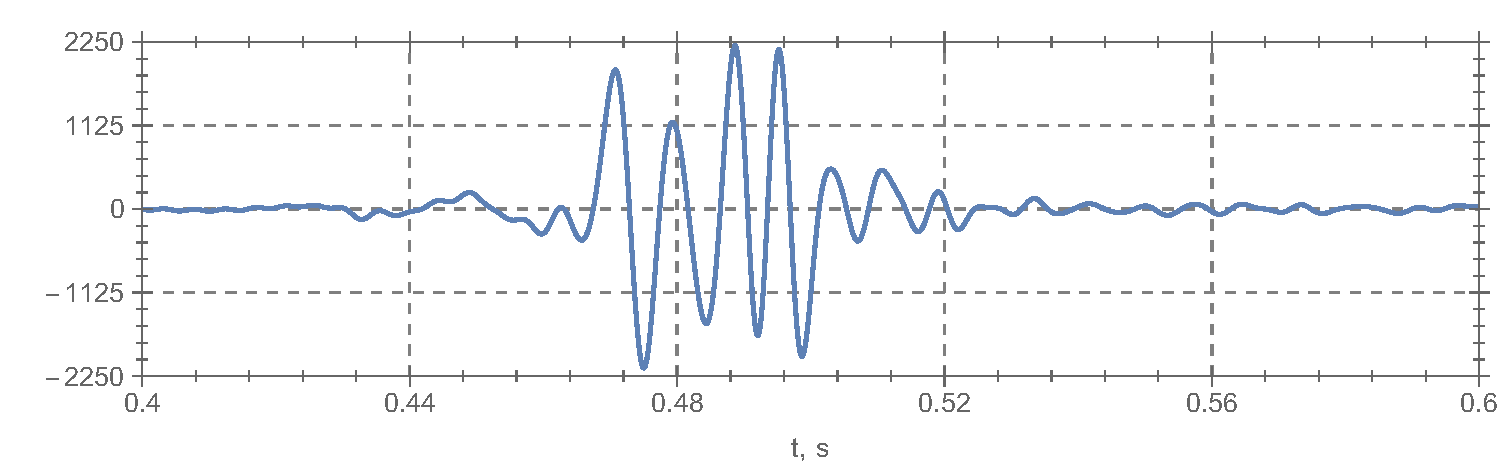
\includegraphics[width=0.7\textwidth]{impulse.pdf}
             \caption{Сигнал во временной области}
         \end{figure}
     \end{frame}

 	\note{Также может быть рассмотрена задача вычисления временного ряда импульса звукового сигнала в произвольных точках среды. Пусть источник излучает сигнал $g\pa{t}$. Тогда импульс $I$ в приёмнике может быть вычислен в спектральной (частотной) области. Здесь $p$ это решение уравнения Гельмгольца для частоты $f$, $\tau$ --- время, которое требуется звуку для достижения приёмника. Также может быть вычислен Sound Exposure Level, который является интегралом модуля квадрата звукового давления при диапазоне рассматриваемых частот $f_1, f_2$ и обозначает уровень шума в данной точке}

 	\begin{frame}[fragile]{Обзор существующих решений}
         \begin{block}{Лучевая теория распространения звука}
             \begin{itemize}
                 \item BELLHOP
                 \item Traceo3D
             \end{itemize}
         \end{block}
         \begin{block}{Трёхмерное параболическое уравнение}
             \begin{itemize}
                 \item Закрытые программные продукты Океанографического института в Вудс-Хоуле и центральной школы Лиона
             \end{itemize}
         \end{block}
         \begin{block}{}
             \begin{itemize}
                 \item[\large\color{greenish}+] Высокая точность
                 \item[\large\color{redish}\textminus] Низкая скорость работы
                 \item[\large\color{redish}\textminus] Большие затраты памяти
             \end{itemize}
         \end{block}
 	\end{frame}

 	\note{На данный момент существует несколько программных продуктов позволяющих вычислять численное решение уравнения Гельмгольца. BELLHOP и Traceo3D основанны на лучевой теории распространения звука. Океанографический институт в Вудс-Хоуле и центральная школа Лиона имеют закрытые комплексы программ, основанные на решении трёхмерного параболического уравнения. Недостатком этих методов являются большие затраты памяти и времени, расчёт самых простых задач занимает не менее суток.}

 	\begin{frame}{Входные и выходные данные}
 		\begin{block}{Входные данные}
 			\begin{itemize}
 				\item config.json
 				\item Дополнительные текстовые или бинарные файлы
 				\vspace{-0.25cm}
 				\begin{multicols}{2}
 					\begin{itemize}
 						\item Модовые функции и собственные значения
 						\item Частоты
 						\item Батиметрия
 					\end{itemize}
 					\columnbreak
 					\begin{itemize}
 						\item Гидрология
 						\item Координаты приёмников
 						\item Функция и спектр источника
 					\end{itemize}
 				\end{multicols}
 			\end{itemize}
 		\end{block}
 		\begin{block}{Выходные данные}
 			\begin{itemize}
 				\item meta.json
 				\item config.json
 				\item Файлы вывода
 				\item Папки вывода нескольких фалов {\small\ttfamilylatin <job\_type>/meta.json}
 			\end{itemize}
 		\end{block}
 	\end{frame}

 	\note{Основным входным файлом программы является конфигурационный файл, который позволяет задавать параметры среды, источника и приёмников. Выходными данными являются несколько файлов в формате JSON, описывающие информацию о проведённых вычислениях, использованных параметрах, а также описание многомерных данных, полученных в результате работы. Этим могут является звуковое поле источника, начальные условия, модовые функции и волновые числа, импульс звукового сигнала, SEL, координаты распространения лучей}
    
     \begin{frame}[fragile]{Волновод Пекериса}
         \begin{figure}[h]
             \centering
             \begin{subfigure}[t]{0.35\textwidth}
                 \centering
                 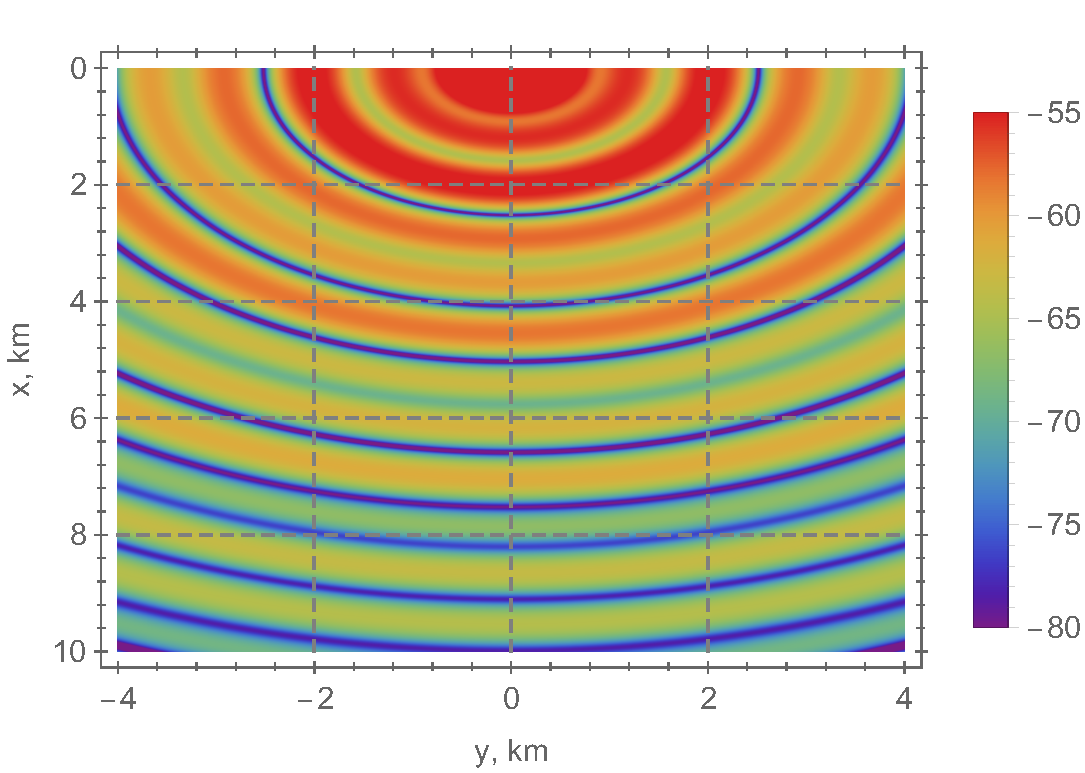
\includegraphics[width=\textwidth]{pekeris.pdf}
                 \caption{Аналитическое решение}
             \end{subfigure}
             \begin{subfigure}[t]{0.35\textwidth}
                 \centering
                 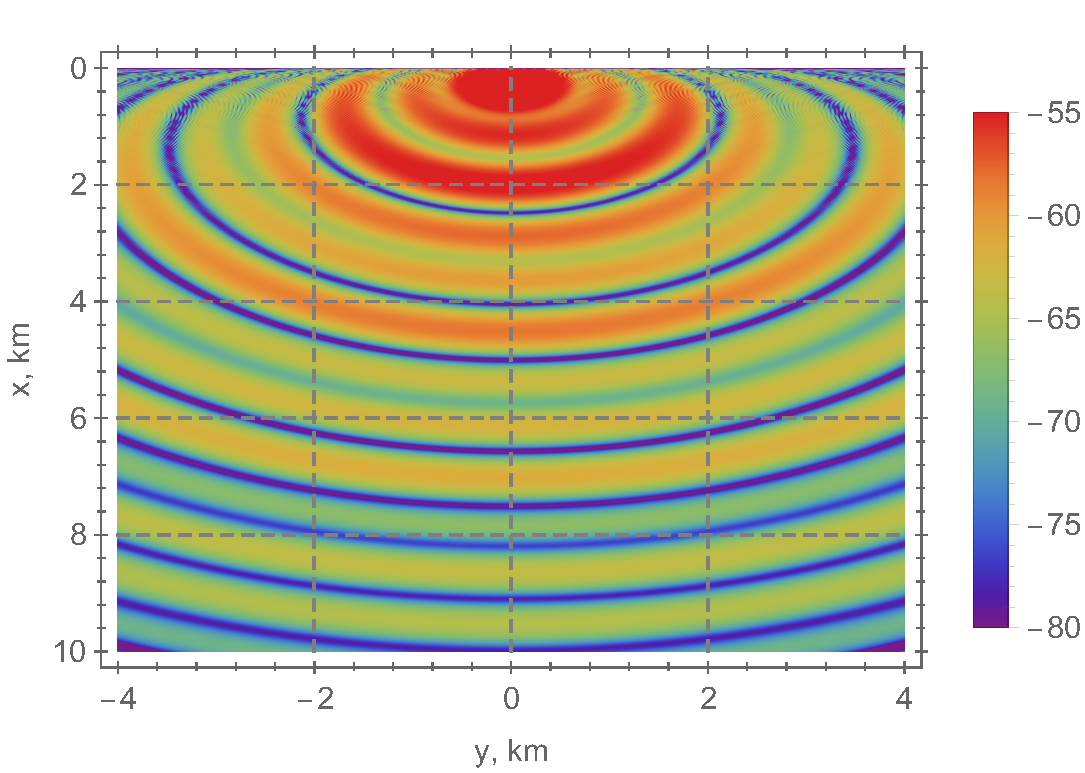
\includegraphics[width=\textwidth]{pekeris_wampe.pdf}
                 \caption{Решение ШМПУ}
             \end{subfigure}\\
             \begin{subfigure}[t]{0.35\textwidth}
                 \centering
                 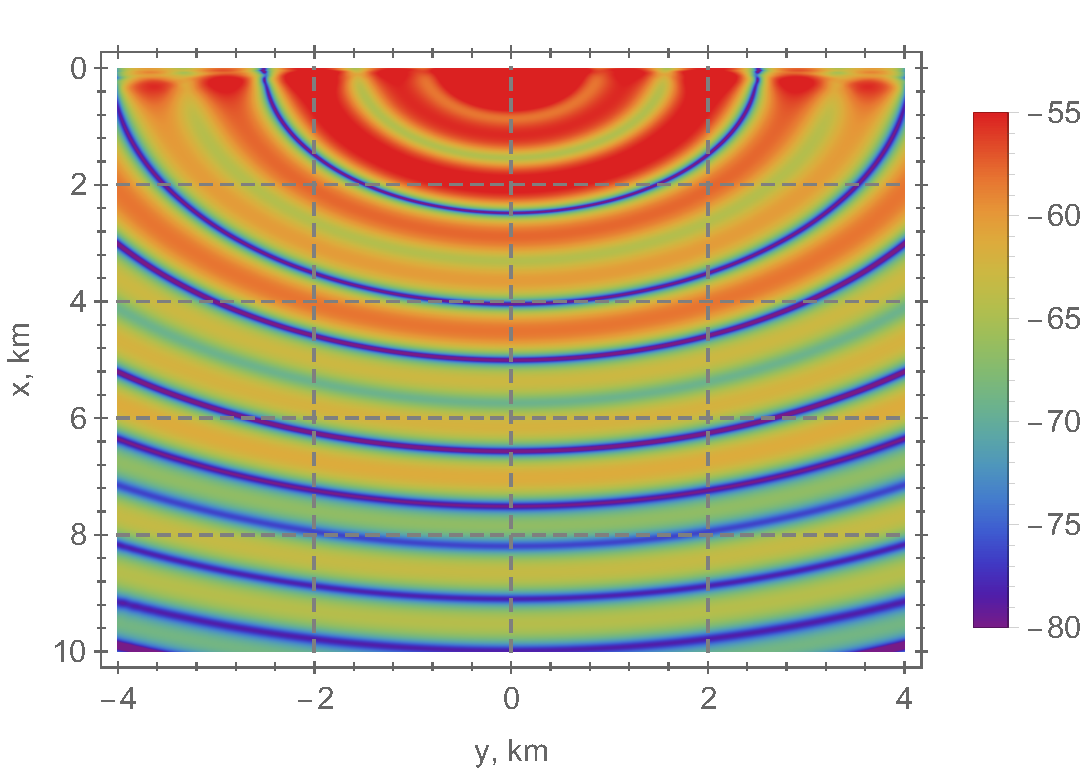
\includegraphics[width=\textwidth]{pekeris_n5.pdf}
                 \caption{SSP, $p=5$}
             \end{subfigure}
             \begin{subfigure}[t]{0.35\textwidth}
                 \centering
                 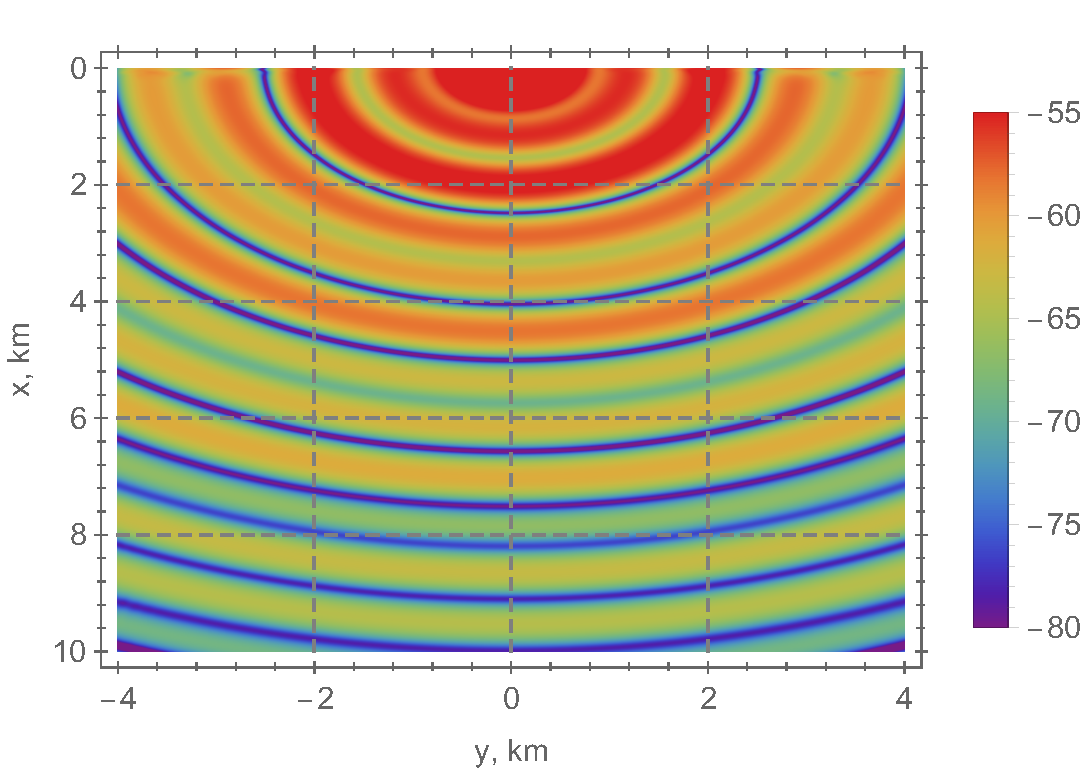
\includegraphics[width=\textwidth]{pekeris_n17.pdf}
                 \caption{SSP, $p=17$}
             \end{subfigure}
             \caption{Акустическое поле в волноводе Пекериса}
         \end{figure}
     \end{frame}

     \note{В качестве первого эксперимента было проведено моделирование распространения звука в волноводе с постоянной глубиной дна. Полученное решение сравнивалось с аналитическим решением и решением ШМПУ с использованием аппроксимации Клаербоута квадратного корня и начальных условий Грина. Как видно из рисунка использование SSP метода с простыми лучевыми начальными условиями и большим порядком аппроксимации позволяет получить решение, которое почти идеально аппроксимирует аналитическое}
    
     \begin{frame}[fragile]{Принцип работы PML граничных условий}
         \begin{figure}[h]
             \centering
             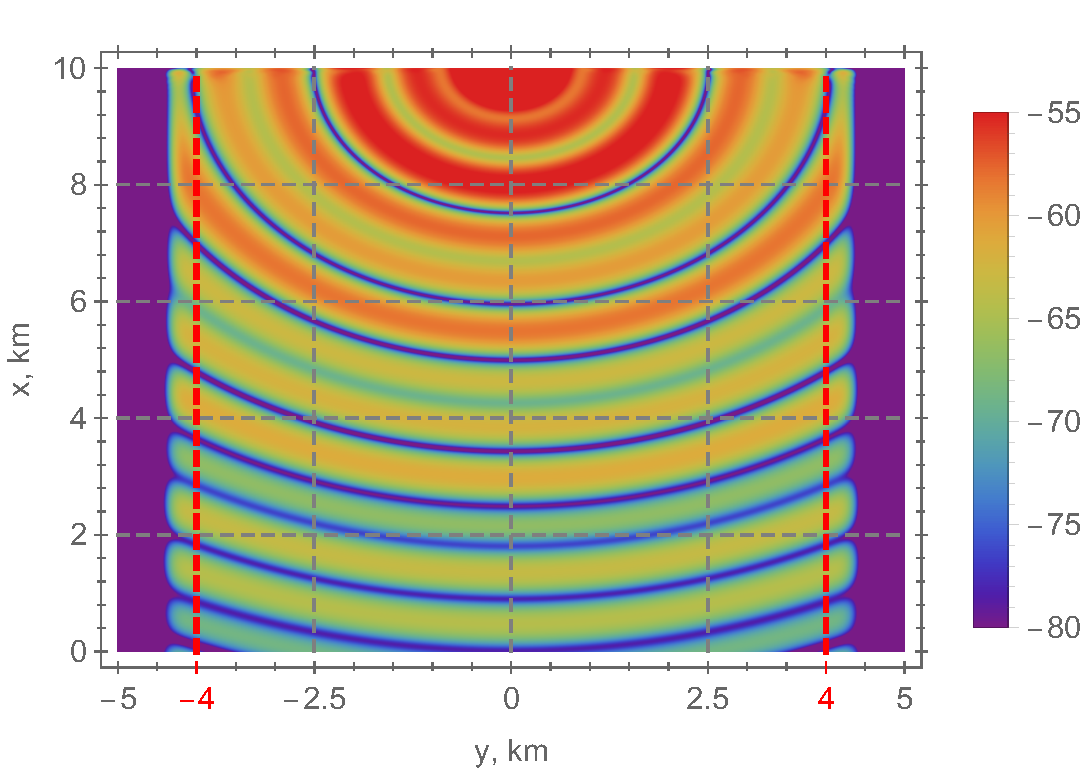
\includegraphics[width=0.7\textwidth]{pekeris_pml_n13.pdf}
             \caption{Акустическое поле в волноводе Пекериса на глубине $z=30\ \text{м.}$, слои PML отмечены красной пунктирной линией, ширина слоёв составляет $1$ километр, порядок аппроксимации Падэ $p=13$}
         \end{figure}
     \end{frame}

     \note{Также была изучена работа PML граничных условий, так, исходящие из вычислительной области волны постепенно затухают при движении вглубь поглощающего слоя}

     \begin{frame}[fragile]{Подводный каньон}
         \vspace{-0.25cm}
         \begin{figure}[h]
             \centering
             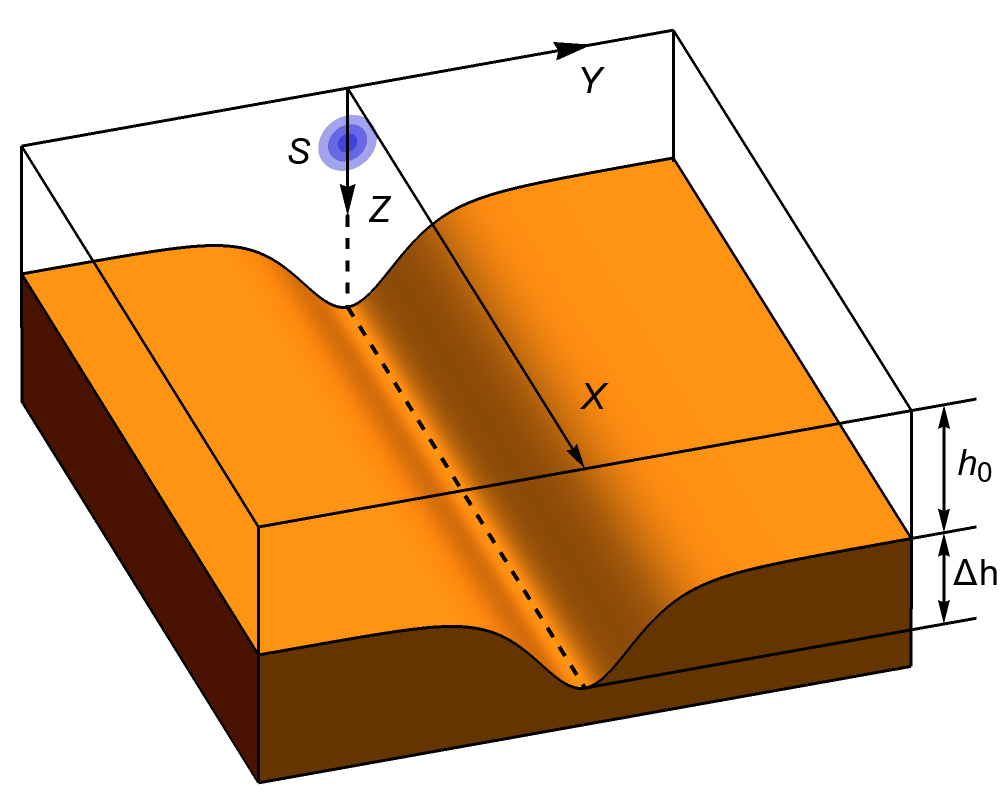
\includegraphics[width=0.3\textwidth]{canyon_transparent.png}
             \caption{Схематичное изображение волновода}
         \end{figure}
         \vspace{-0.75cm}
         \begin{figure}[h]
             \centering
             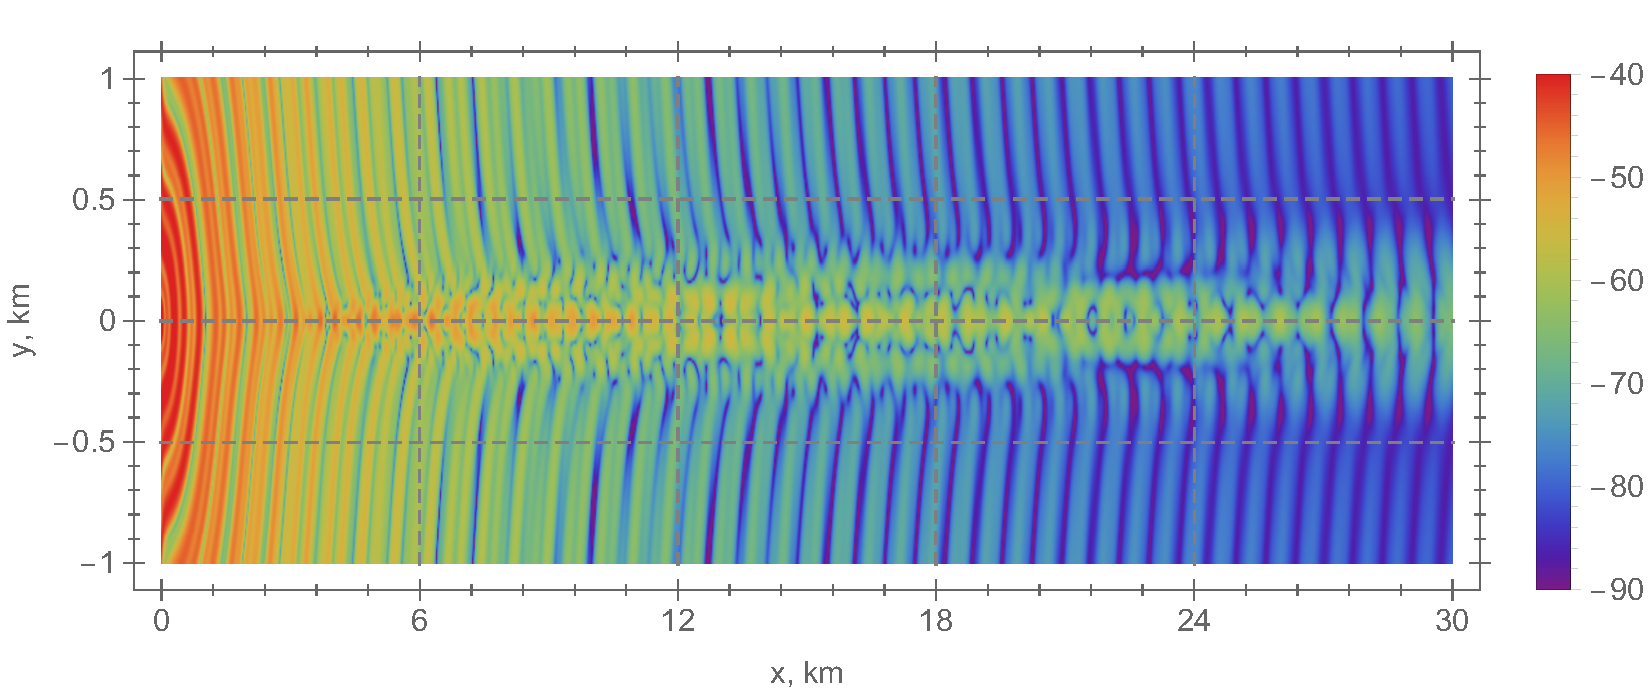
\includegraphics[width=0.75\textwidth]{canyon_n11.pdf}
             \caption{Акустическое поле в волноводе с подводным каньоном}
         \end{figure}
     \end{frame}

 	\note{Далее был рассмотрен подводный каньон. Решение было получено с использованием 11 членов аппроксимации и простых лучевых начальных условий. Как видно из рисунка, полученное решение имеет апертуру почти $\pm 90^\circ$}
    
     \begin{frame}[fragile]{Подводный каньон. Сравнительный анализ}
         \begin{figure}[h]
             \centering
             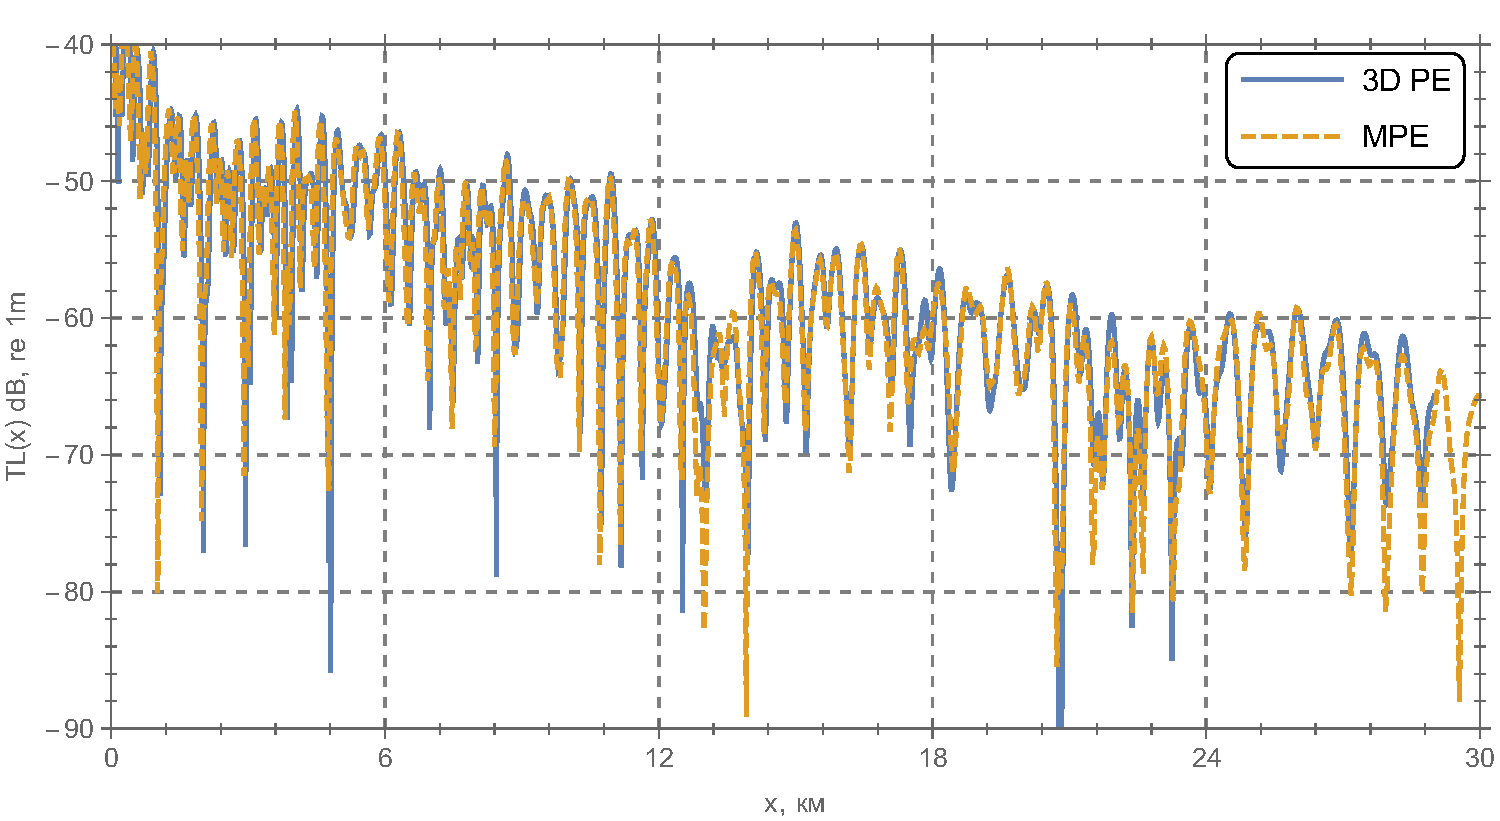
\includegraphics[width=0.9\textwidth]{canyon_compare.pdf}
             \caption{Сравнение результатов вычисления акустического поля в мелком море с подводным каньоном при $y=0\ \text{км.}$ на глубине $z=10\ \text{м}$.}
         \end{figure}
     \end{frame}

     \note{Полученное решение также сравнивалось с решением трёхмерного параболического уравнения при $y=0$ на глубине $10$ метров. Из рисунка видно, что решения достаточно сильно совпадают, при этом решение МПУ требует значительно меньше вычислительных ресурсов}

 	\begin{frame}{Подводный каньон. Трассировка лучей}
 		\begin{figure}[h]
 			\centering
             \begin{subfigure}{0.45\textwidth}
                 \centering
                 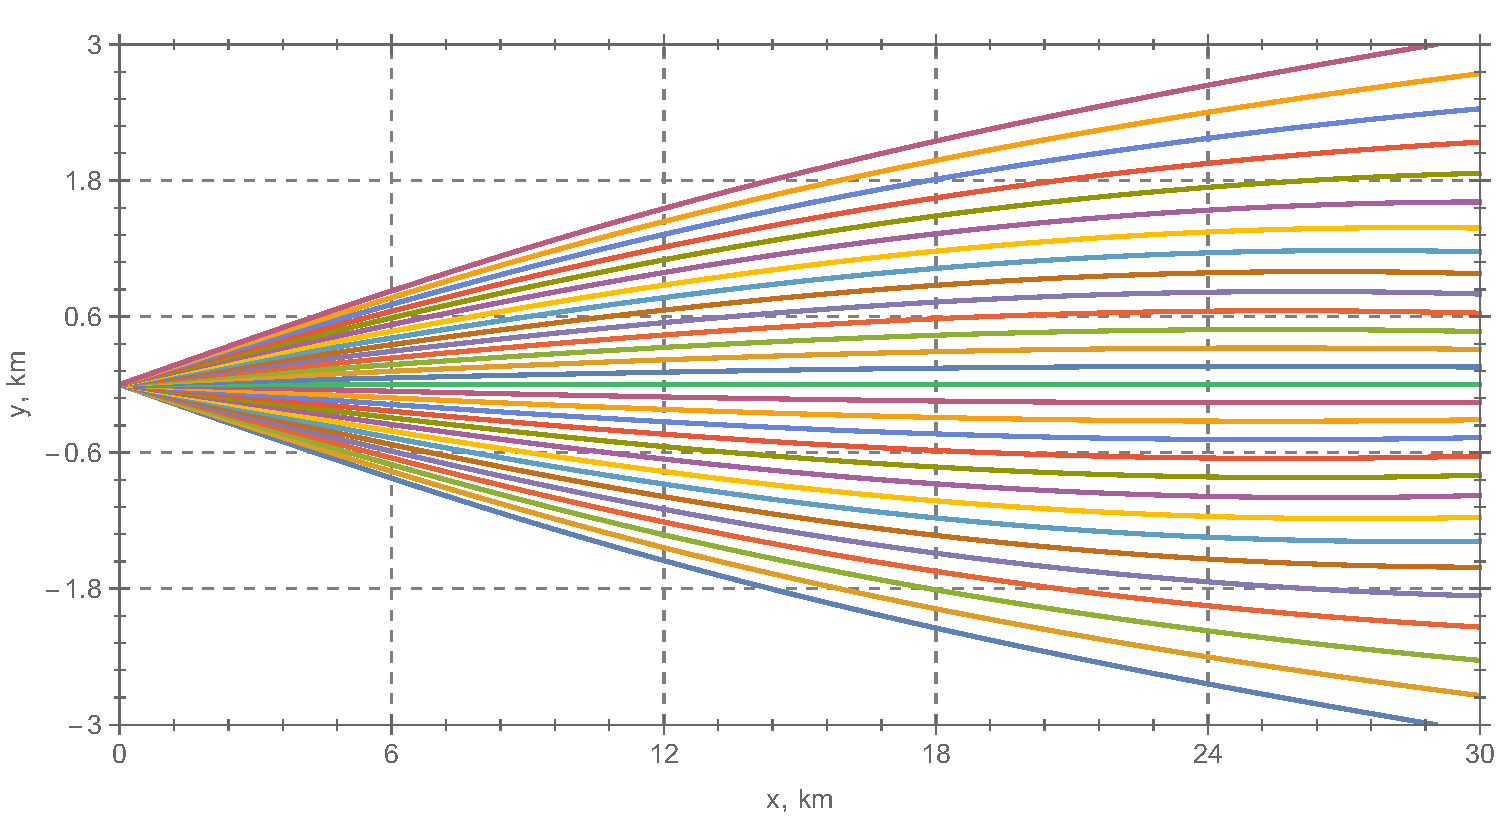
\includegraphics[width=\textwidth]{canyon_rays_1.pdf}
                 \caption{1-ая мода}
             \end{subfigure}
             \begin{subfigure}{0.45\textwidth}
                 \centering
                 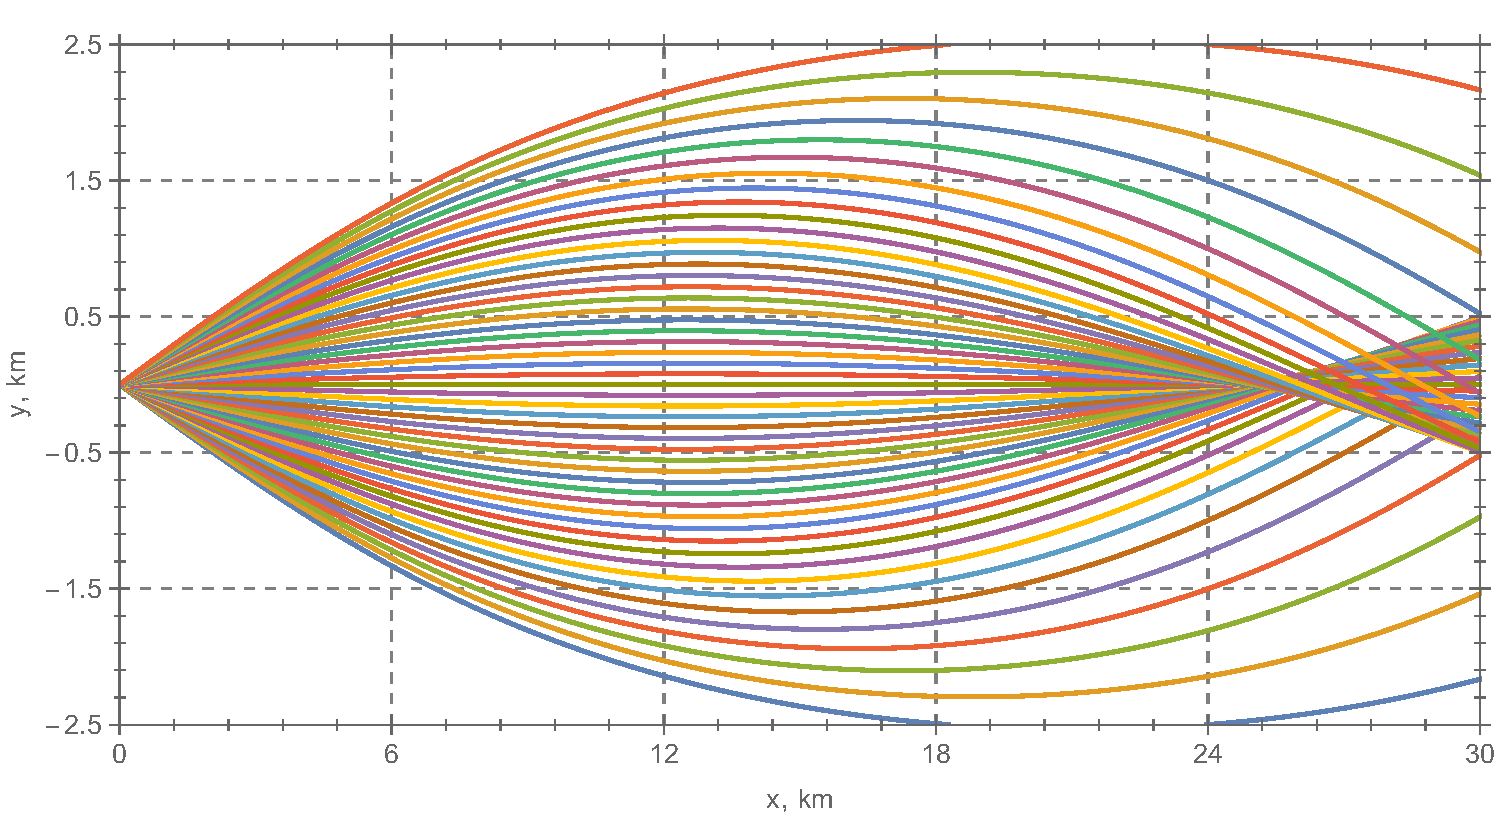
\includegraphics[width=\textwidth]{canyon_rays_2.pdf}
                 \caption{2-ая мода}
             \end{subfigure}\\
             \begin{subfigure}{0.45\textwidth}
                 \centering
                 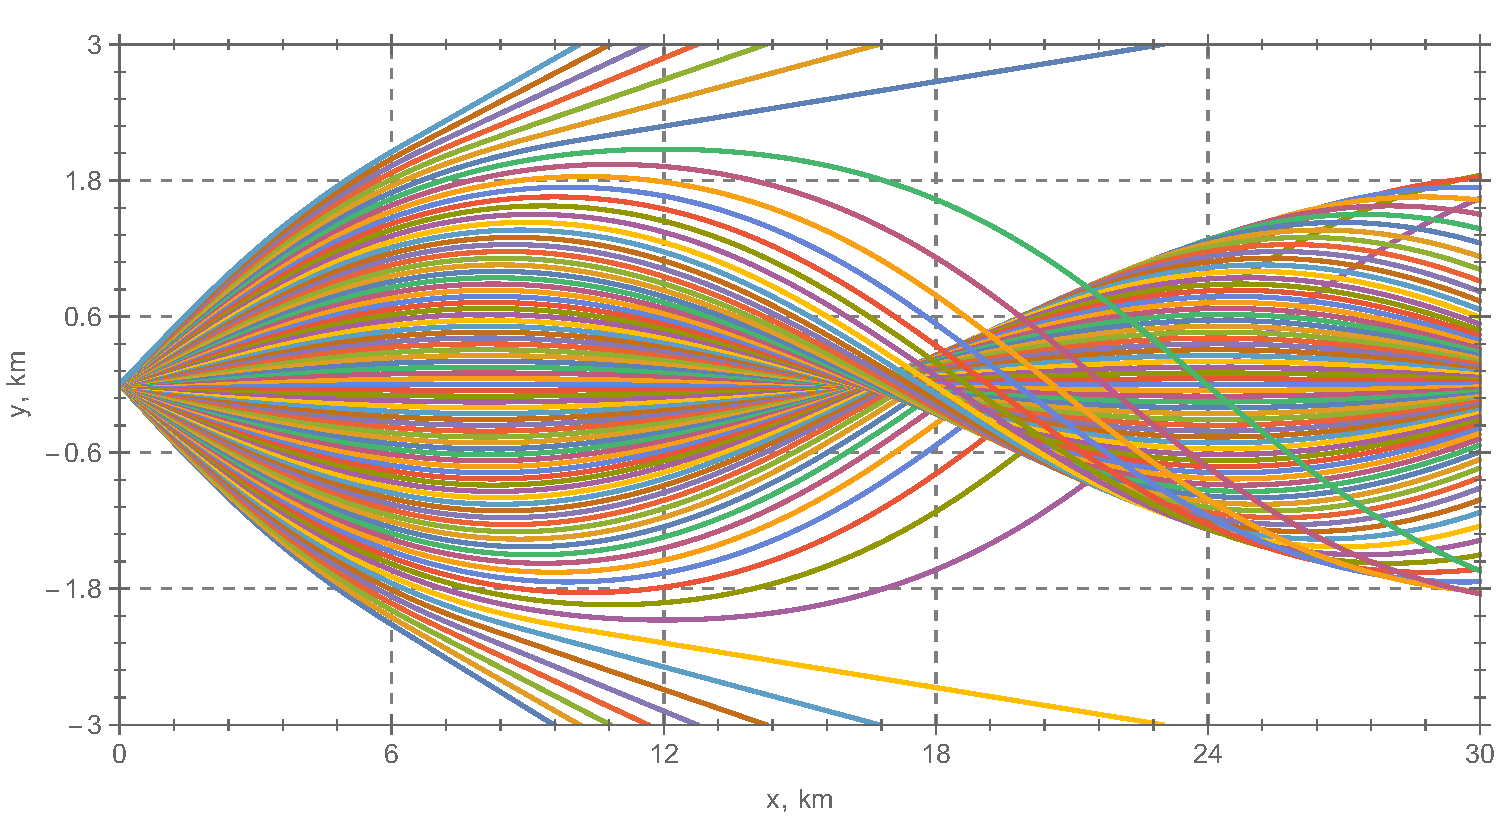
\includegraphics[width=\textwidth]{canyon_rays_3.pdf}
                 \caption{3-ая мода}
             \end{subfigure}
             \begin{subfigure}{0.45\textwidth}
                 \centering
                 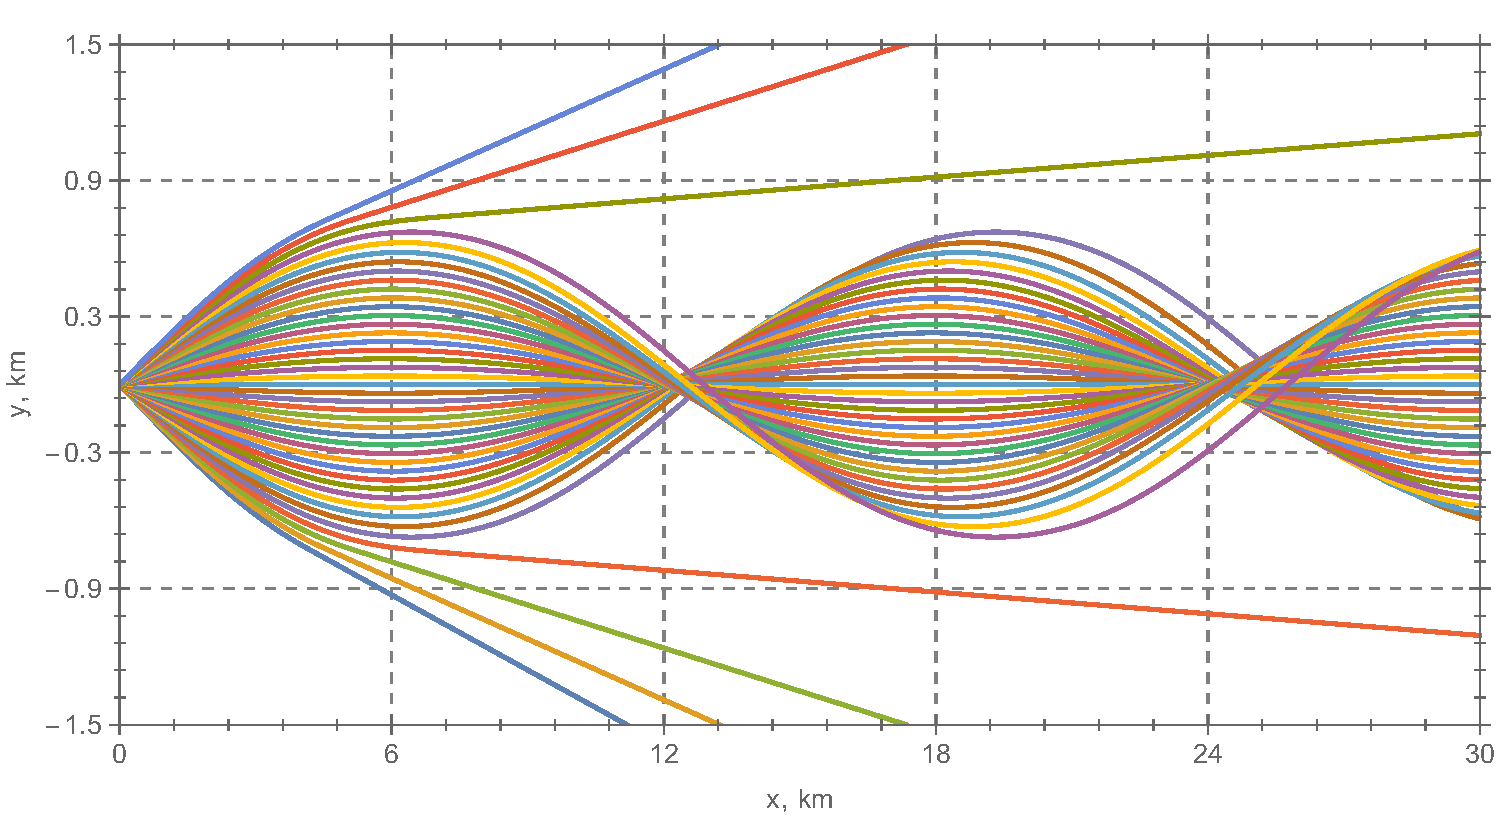
\includegraphics[width=\textwidth]{canyon_rays.pdf}
                 \caption{4-ая мода}
             \end{subfigure}
 			\caption{Лучи, соответствующие вертикальным модам}
 		\end{figure}
 	\end{frame}

 	\note{Также была проведена трассировка лучей, соответствующих вертикальным модам. Каньон захватывает звук, поэтому лучи образуют петли при достаточно небольшом угле отклонения от главной оси распространения. С увеличением номера моды захват становится более выраженным}
    
     \begin{frame}[fragile]{Клиновидный волновод}
         \vspace{-0.25cm}
         \begin{figure}[h]
             \centering
             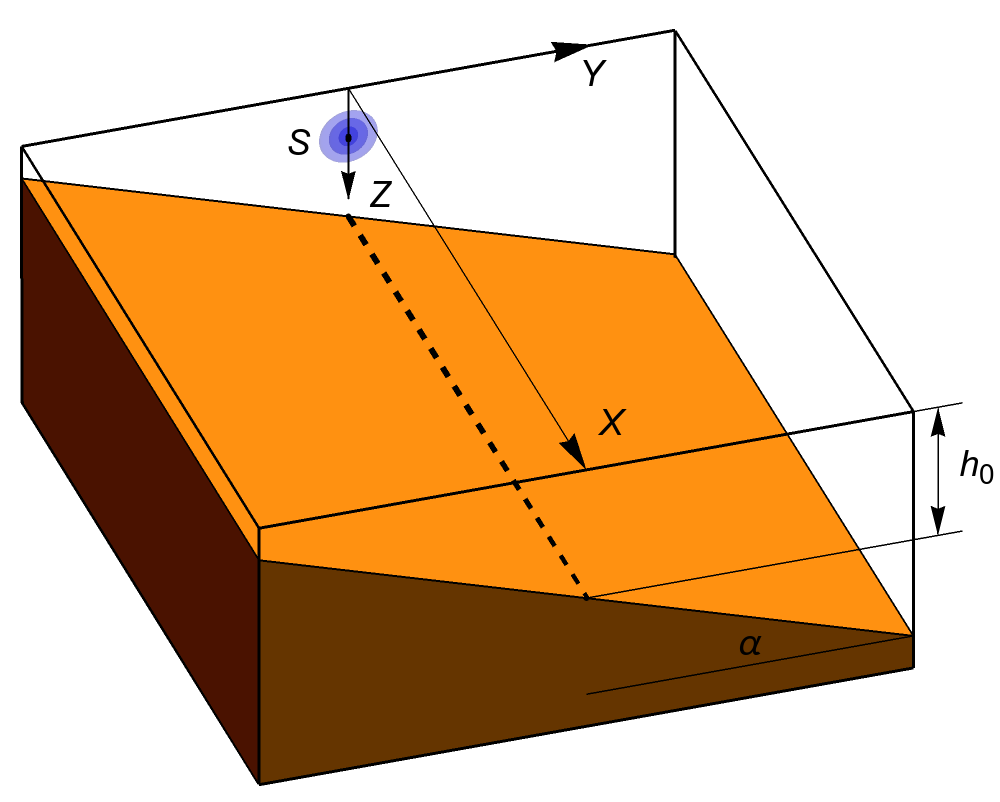
\includegraphics[width=0.3\textwidth]{wedge_transparent.png}
             \caption{Схематичное изображение волновода}
         \end{figure}
         \vspace{-0.75cm}
         \begin{figure}[h]
             \centering
             \begin{subfigure}[t]{0.35\textwidth}
                 \centering
                 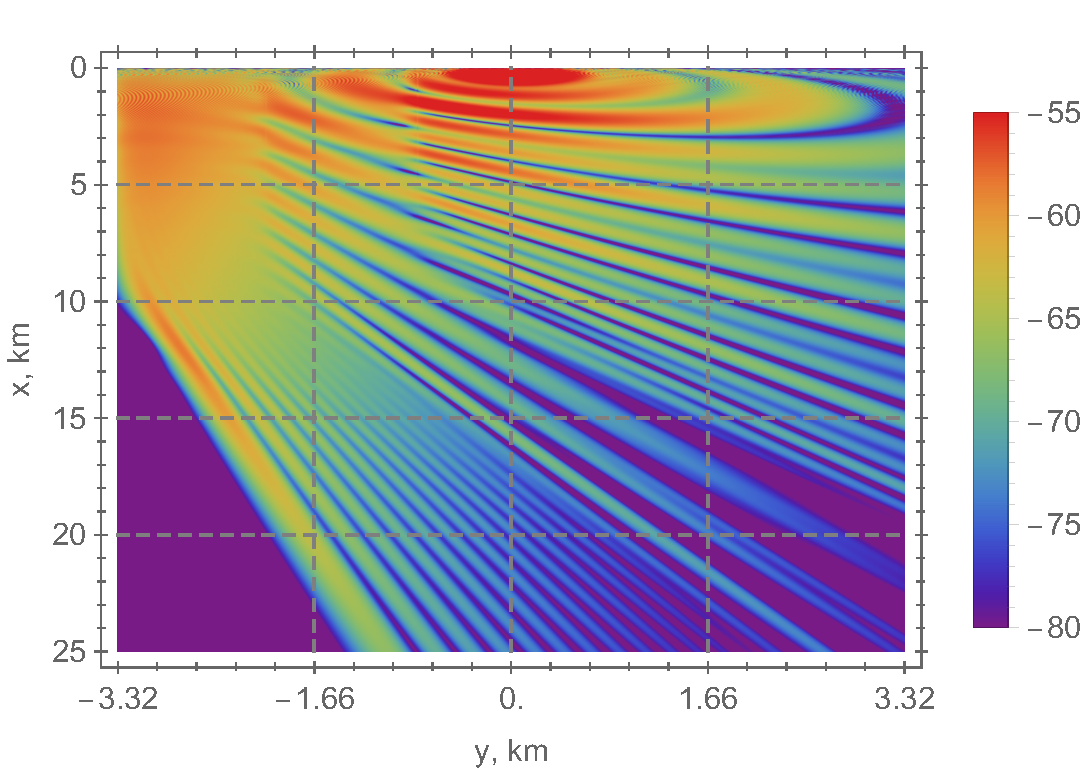
\includegraphics[width=\textwidth]{wedge_wampe.pdf}
                 \caption{Решение ШМПУ}
             \end{subfigure}
             \begin{subfigure}[t]{0.35\textwidth}
                 \centering
                 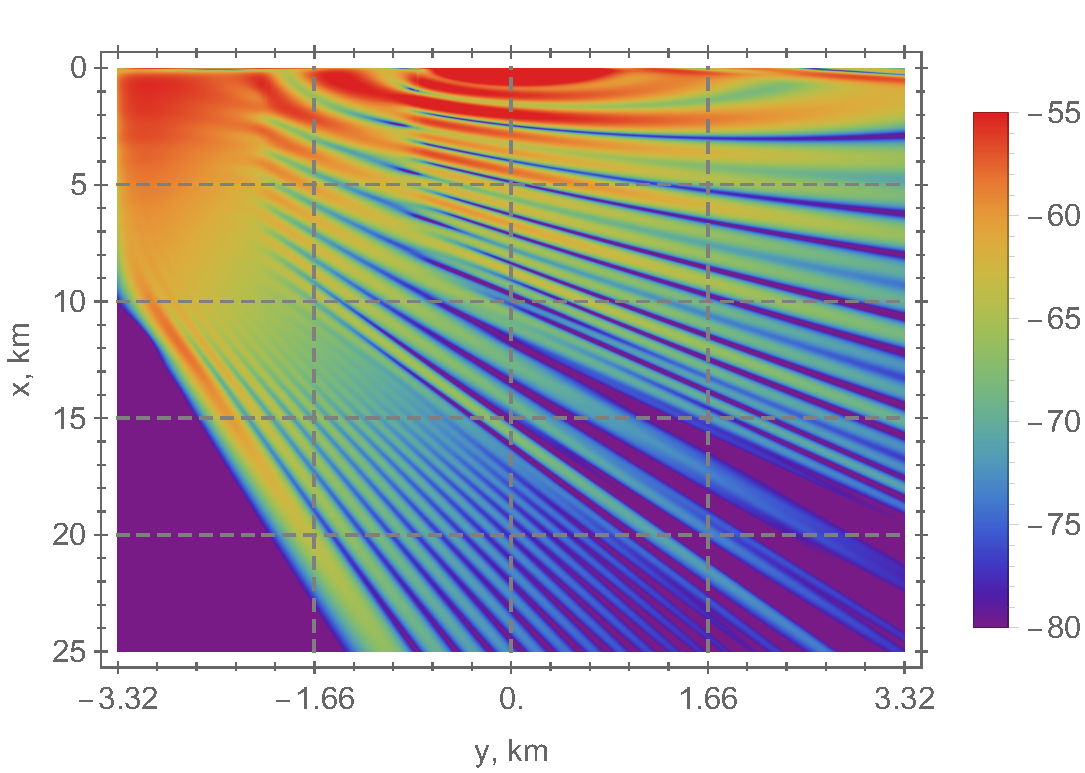
\includegraphics[width=\textwidth]{wedge_n13.pdf}
                 \caption{SSP}
             \end{subfigure}
             \caption{Акустическое поле в клиновидном волноводе}
         \end{figure}
     \end{frame}

     \note{Далее было рассмотрено моделирование распространения звука в клиновидном волноводе.}
    
     \begin{frame}[fragile]{Клиновидный волновод. Сравнительный анализ}
         \begin{figure}[h]
             \centering
             \vspace{-0.25cm}
             \begin{tikzpicture}
                 \node (IMG) at (0,0) {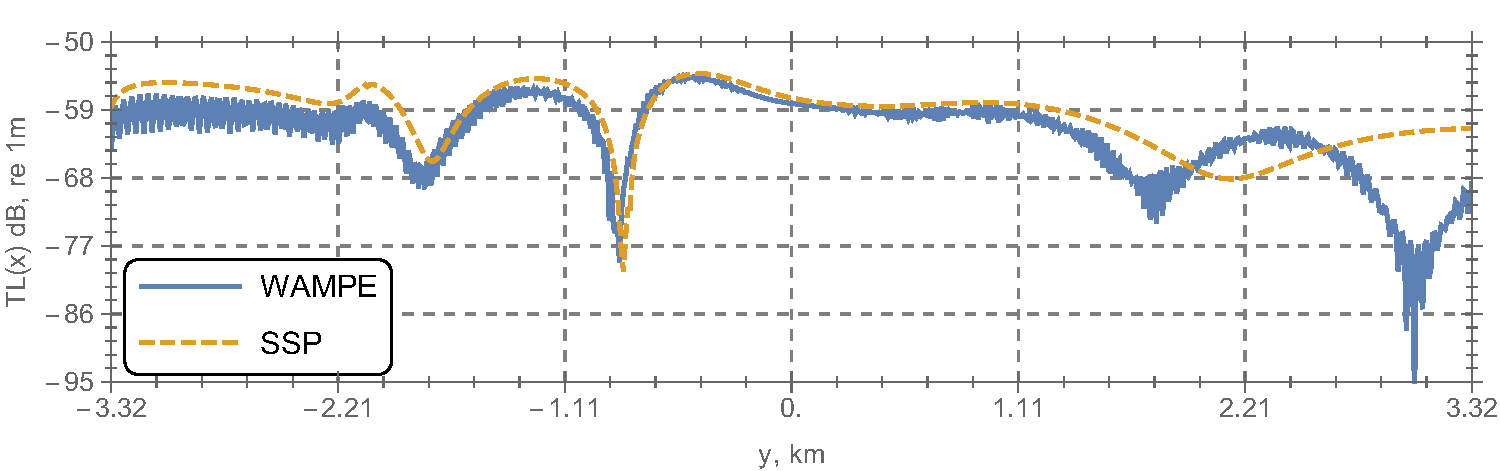
\includegraphics[width=0.6\textwidth]{wedge_comp_1.pdf}};
                 \node[left=.5cm of IMG]{\textbf{(a)} $x=\ 1\ \text{км.}$};
             \end{tikzpicture}
             \begin{tikzpicture}
                 \node (IMG) at (0,0) {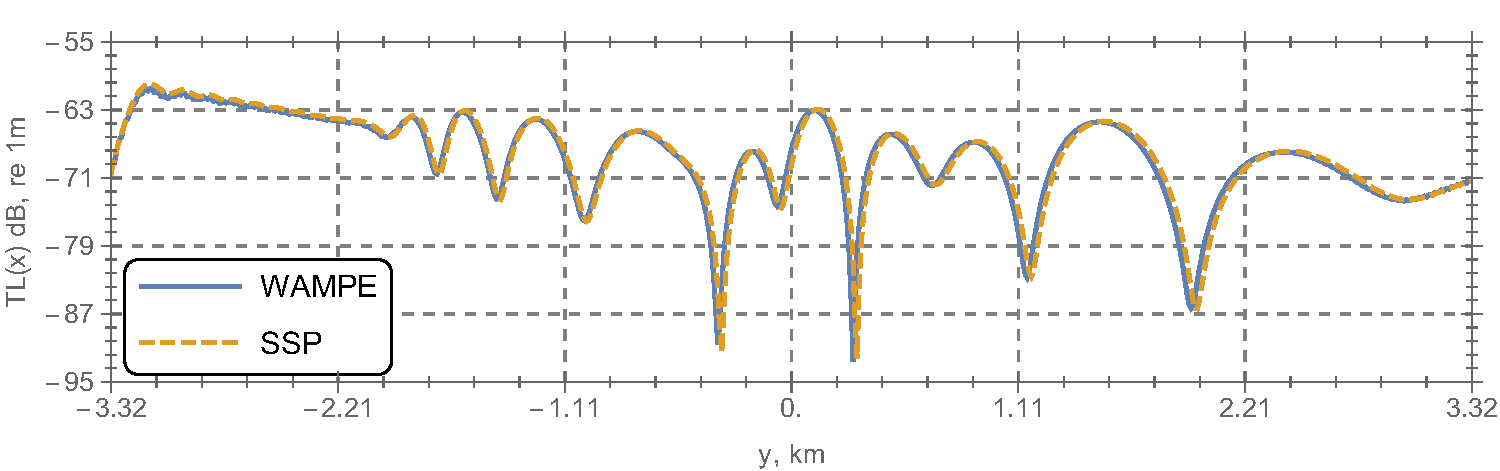
\includegraphics[width=0.6\textwidth]{wedge_comp_9.pdf}};
                 \node[left=.5cm of IMG]{\textbf{(b)} $x=\ 9\ \text{км.}$};
             \end{tikzpicture}
             \begin{tikzpicture}
                 \node (IMG) at (0,0) {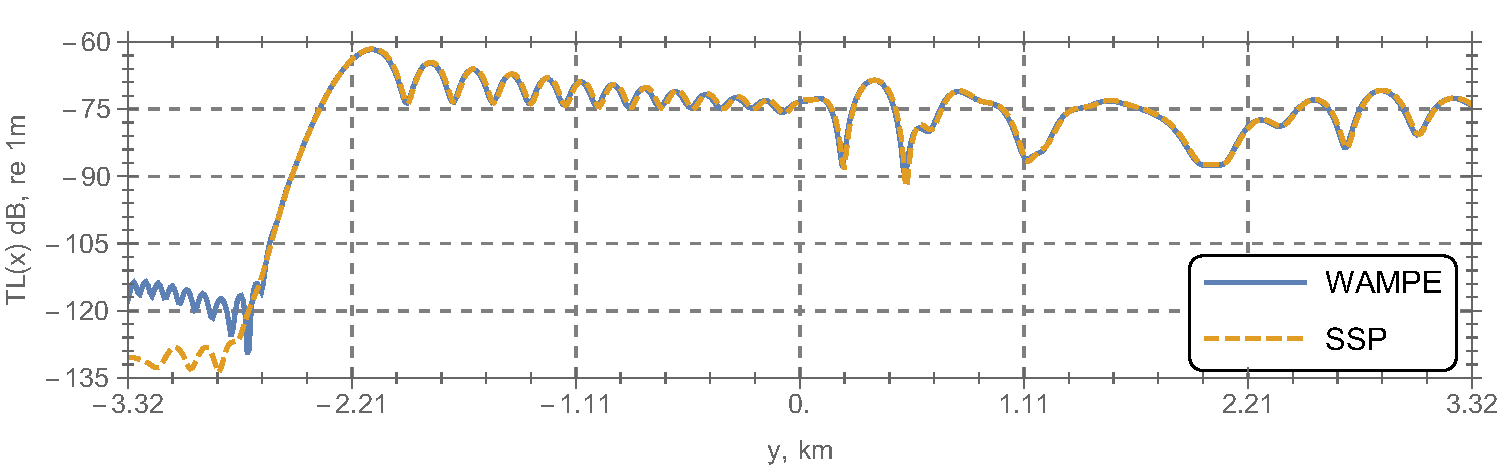
\includegraphics[width=0.6\textwidth]{wedge_comp_17.pdf}};
                 \node[left=.45cm of IMG]{\textbf{(c)} $x=25\ \text{км.}$};
             \end{tikzpicture}
             \caption{Сравнение результатов вычисления акустического поля вдоль $y$}
         \end{figure}
     \end{frame}

     \note{Было произведено сравнения акустического поля на различных горизонтах $x$. Из рисунка видно, что вблизи источника SSP решение не образует численного шума, а при отдалении от источника становится заметна более широкая апертура этого решения.}
    
     \begin{frame}[fragile]{Клиновидный волновод. Сравнительный анализ}
         \begin{figure}[h]
             \centering
             \begin{subfigure}[t]{0.55\textwidth}
                 \centering
                 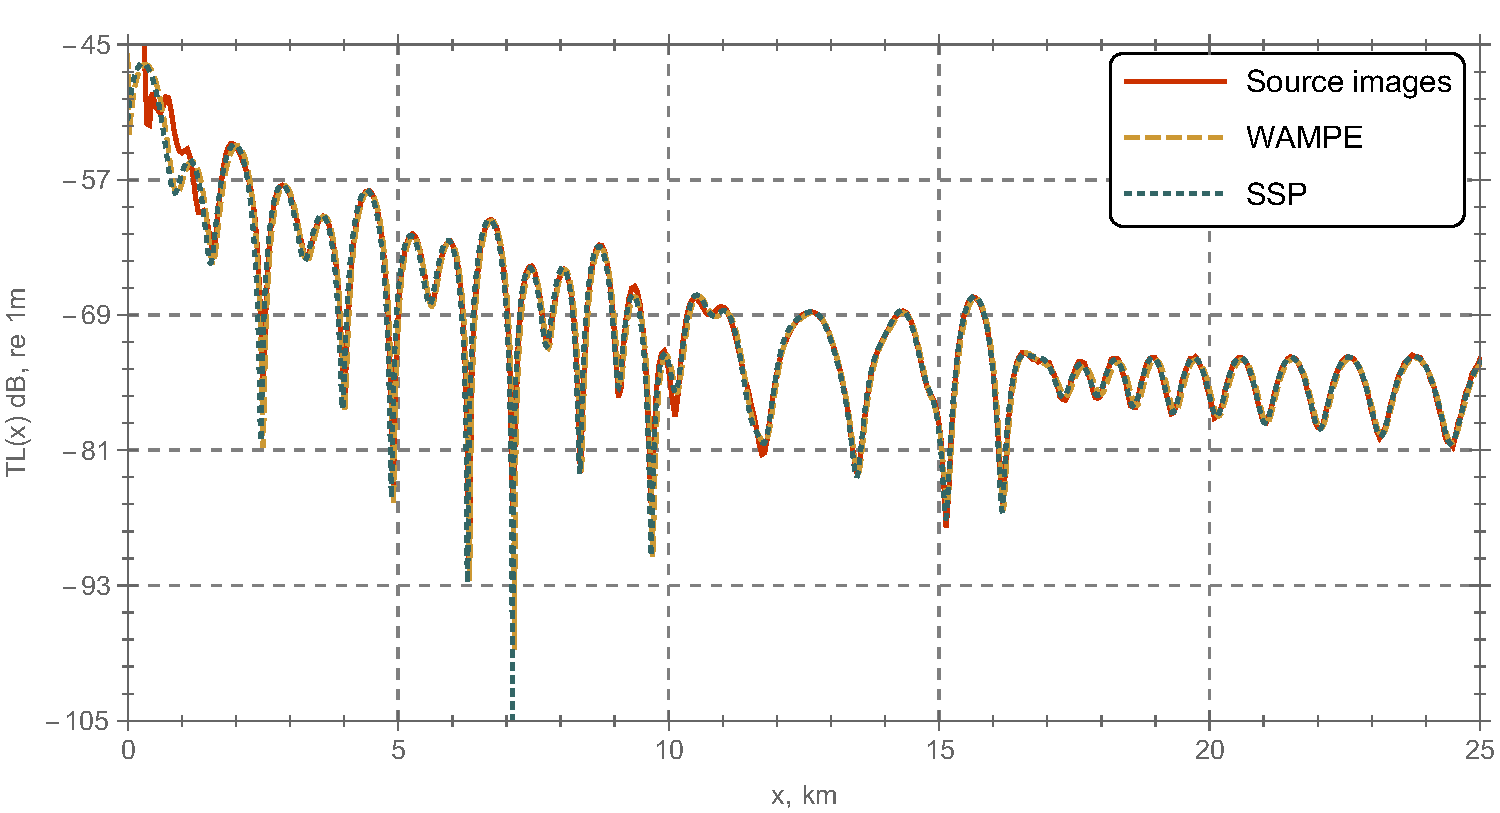
\includegraphics[width=\textwidth]{wedge_comp.pdf}
             \end{subfigure}
             \hfill
             \begin{subfigure}[t]{0.55\textwidth}
                 \centering
                 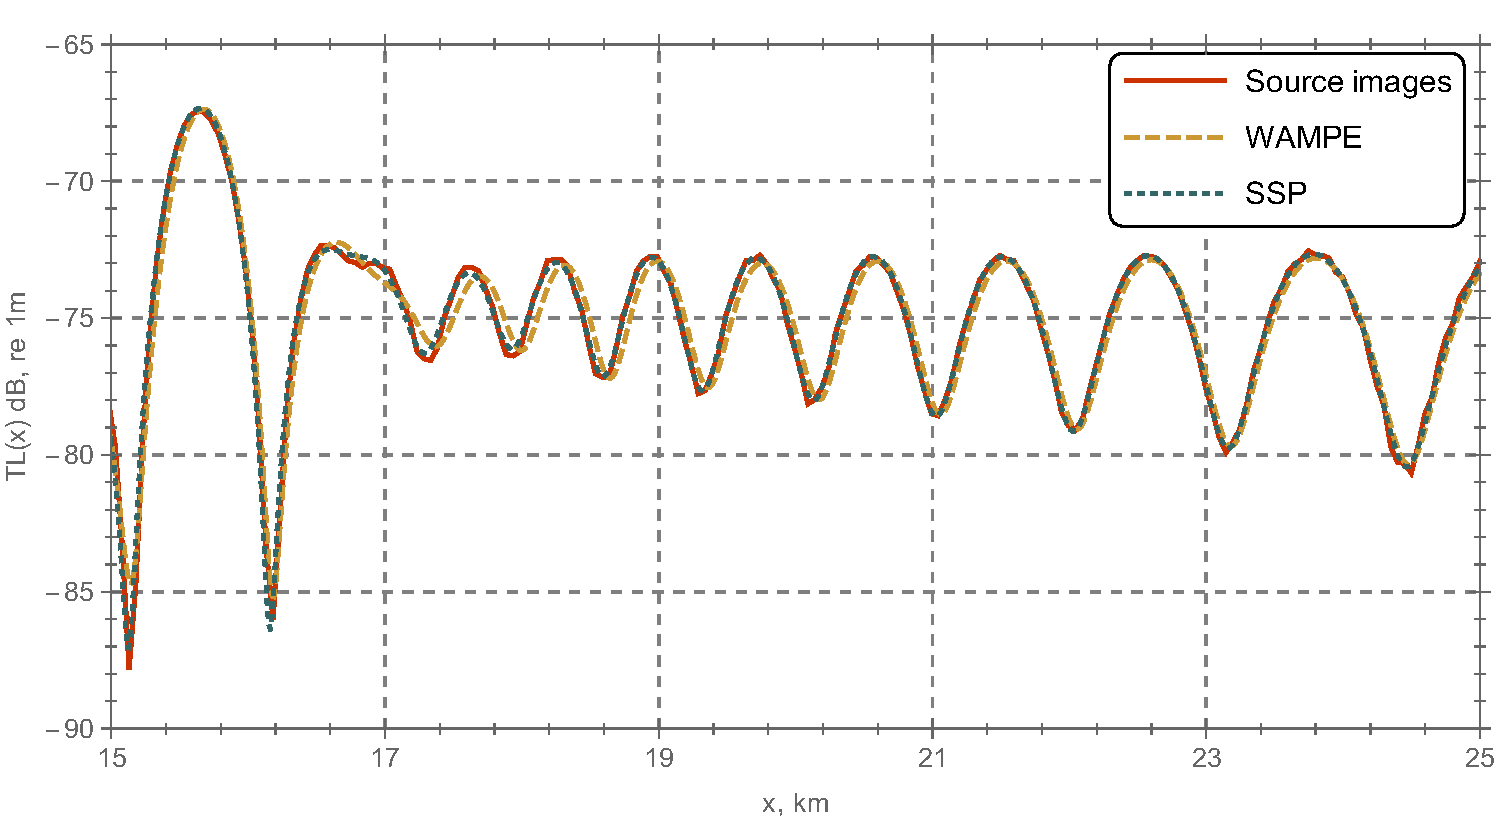
\includegraphics[width=\textwidth]{wedge_comp_close.pdf}
             \end{subfigure}
             \caption{Сравнение результатов вычисления акустического поля вдоль $x$}
         \end{figure}
     \end{frame}

     \note{Также было произведено сравнение с решением методом изображений. Решения всех методов почти совпадают, не смотря на адиабатическую природу модовых параболических уравнений, при этом большая апертура SSP метода сильнее приближает решение к решению методом изображений вдали от источника. Время вычисления решения методом изображений составляет приблизительно 23 часа, по сравнению с несколькими минутами, затрачиваемыми на решение модового параболического уравнения}

     \begin{frame}{Волновод с реальной батиметрией}
         \vspace{-0.25cm}
         \begin{multicols}{2}
             \begin{figure}[h]
                 \centering
                 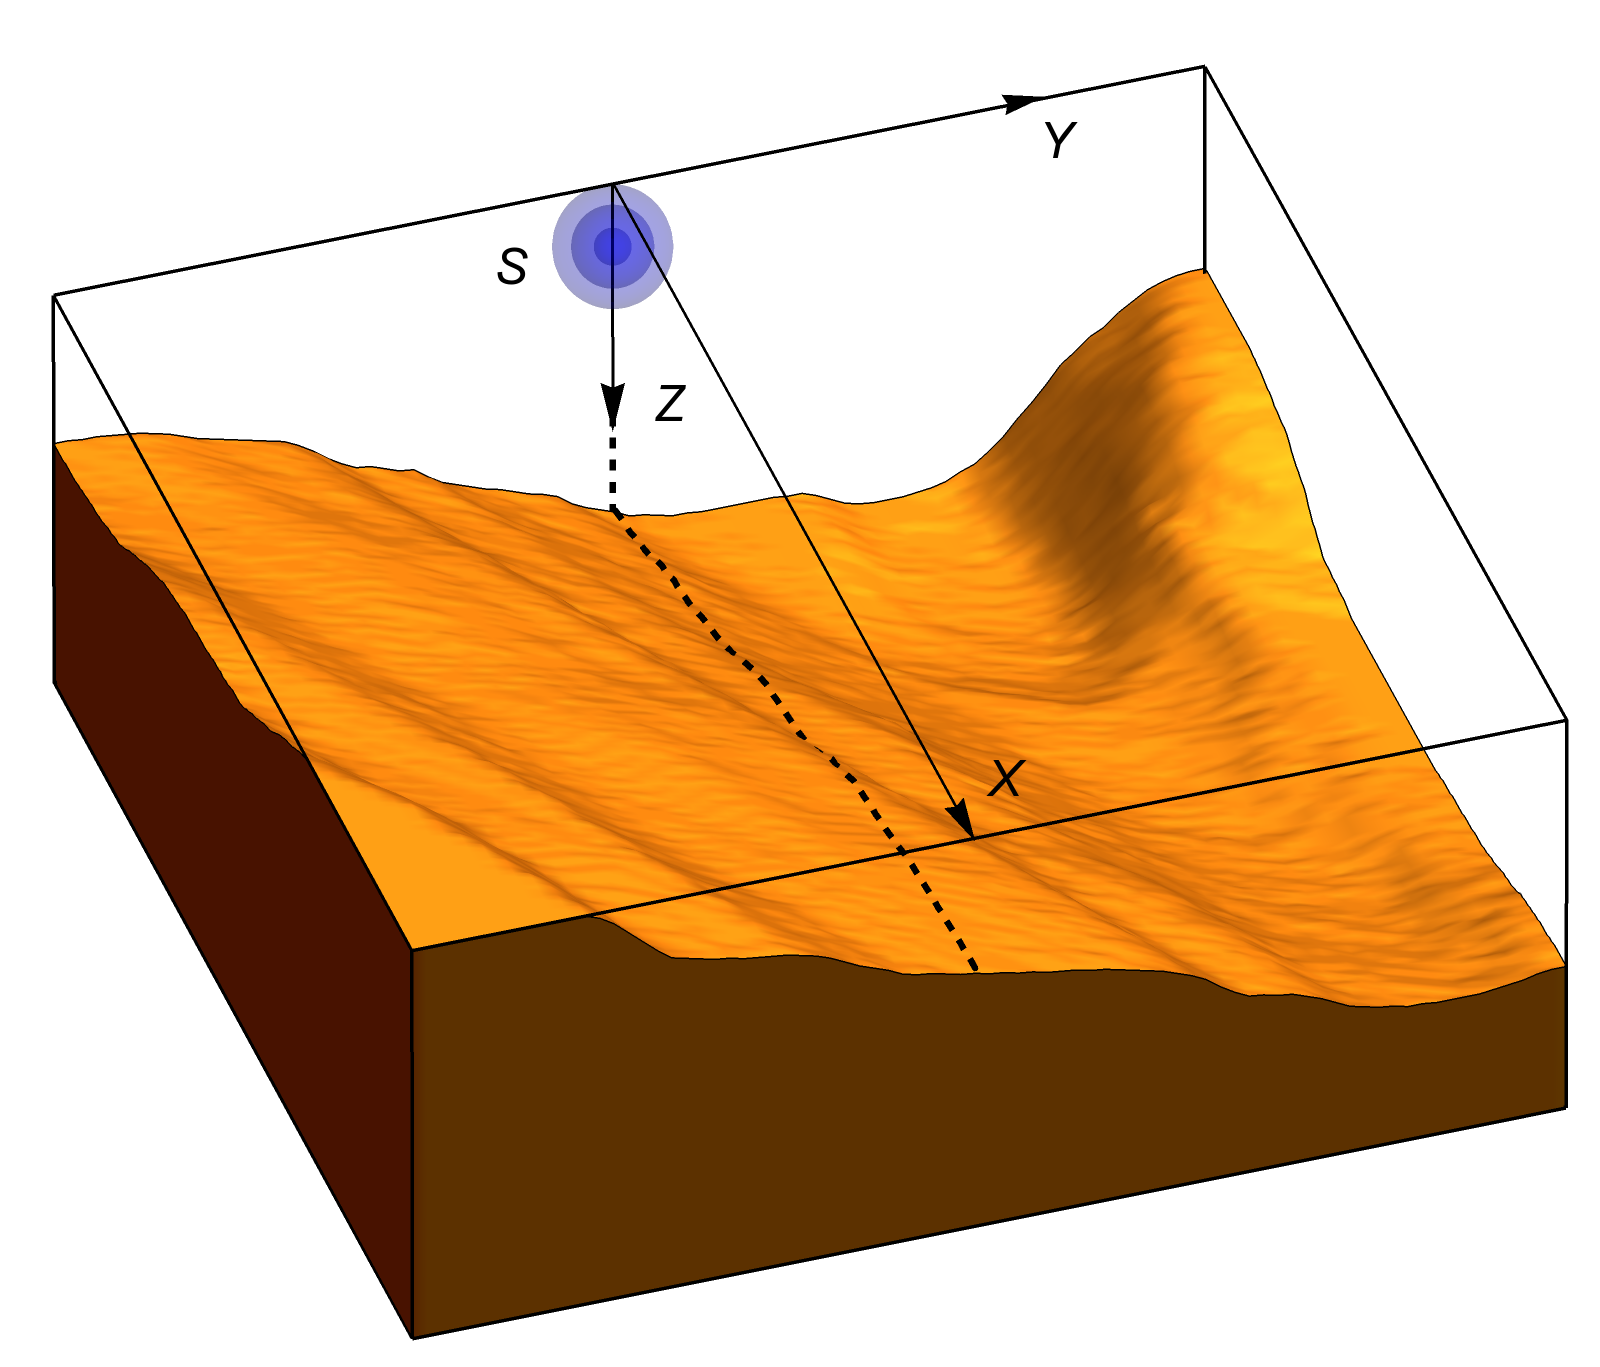
\includegraphics[width=0.4\textwidth]{sakhalin_transparent.png}
                 \caption{Рельеф дна}
             \end{figure}
             \columnbreak
             \begin{figure}[h]
                 \centering
                 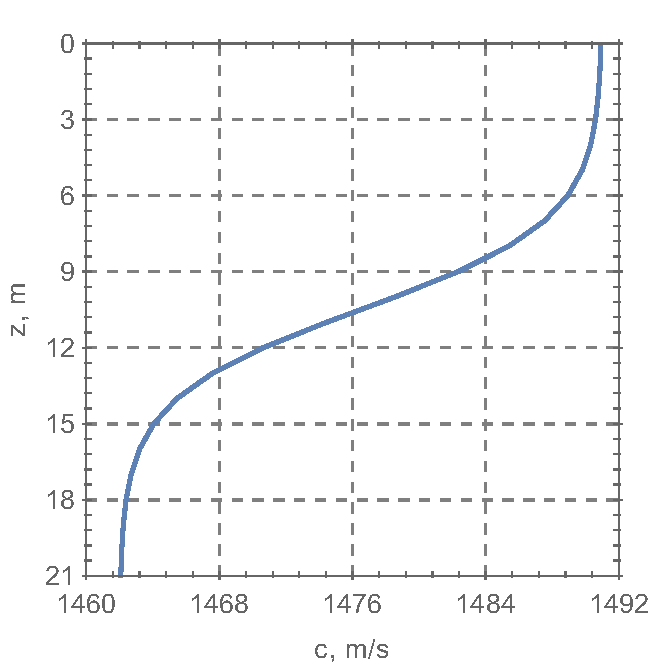
\includegraphics[width=0.33\textwidth]{sound_profile.pdf}
                 \caption{Скорость звука}
             \end{figure}
         \end{multicols}
         \begin{block}{Функция скорости звука}
             \ifmetropolis
                 \smallskip
             \fi
             \begin{equation}
                 c\pa{z}=1491-\frac{29}{1+\exp\pa{6-\frac{12z}{21}}}
             \end{equation}
         \end{block}
     \end{frame}

 	\note{Также была рассмотрена задача с настоящими данными батиметрии и аппроксимацией профиля скорости звука в воде}

 	\begin{frame}[fragile]{\normalsize Волновод с реальной батиметрией. Акустическое поле источника}
 		\begin{figure}[h]
 			\centering
             \begin{subfigure}{.6\textwidth}
                 \centering
                 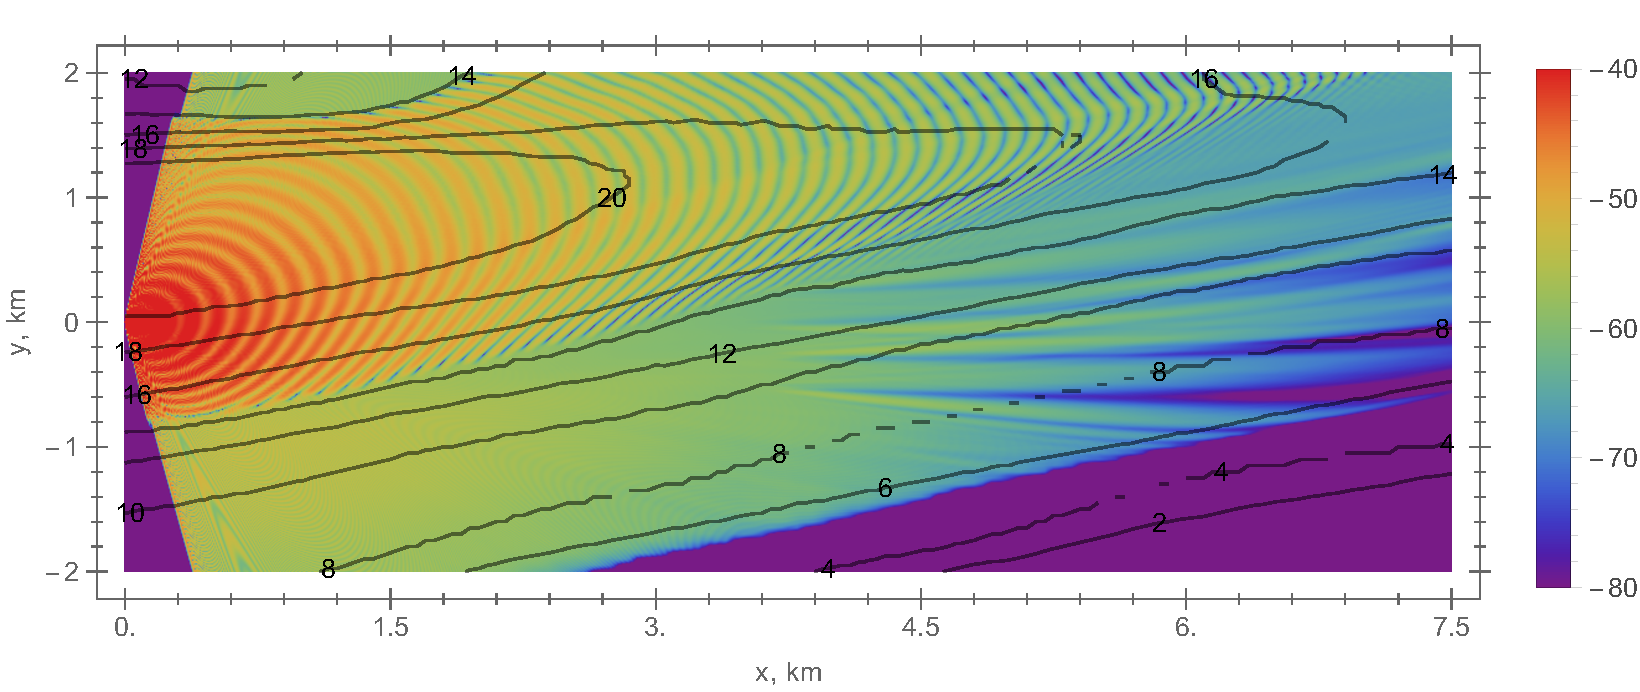
\includegraphics[width=\textwidth]{sakhalin_wampe_z4.pdf}
                 \caption{Решение ШМПУ}
             \end{subfigure}
             \begin{subfigure}{.6\textwidth}
                 \centering
                 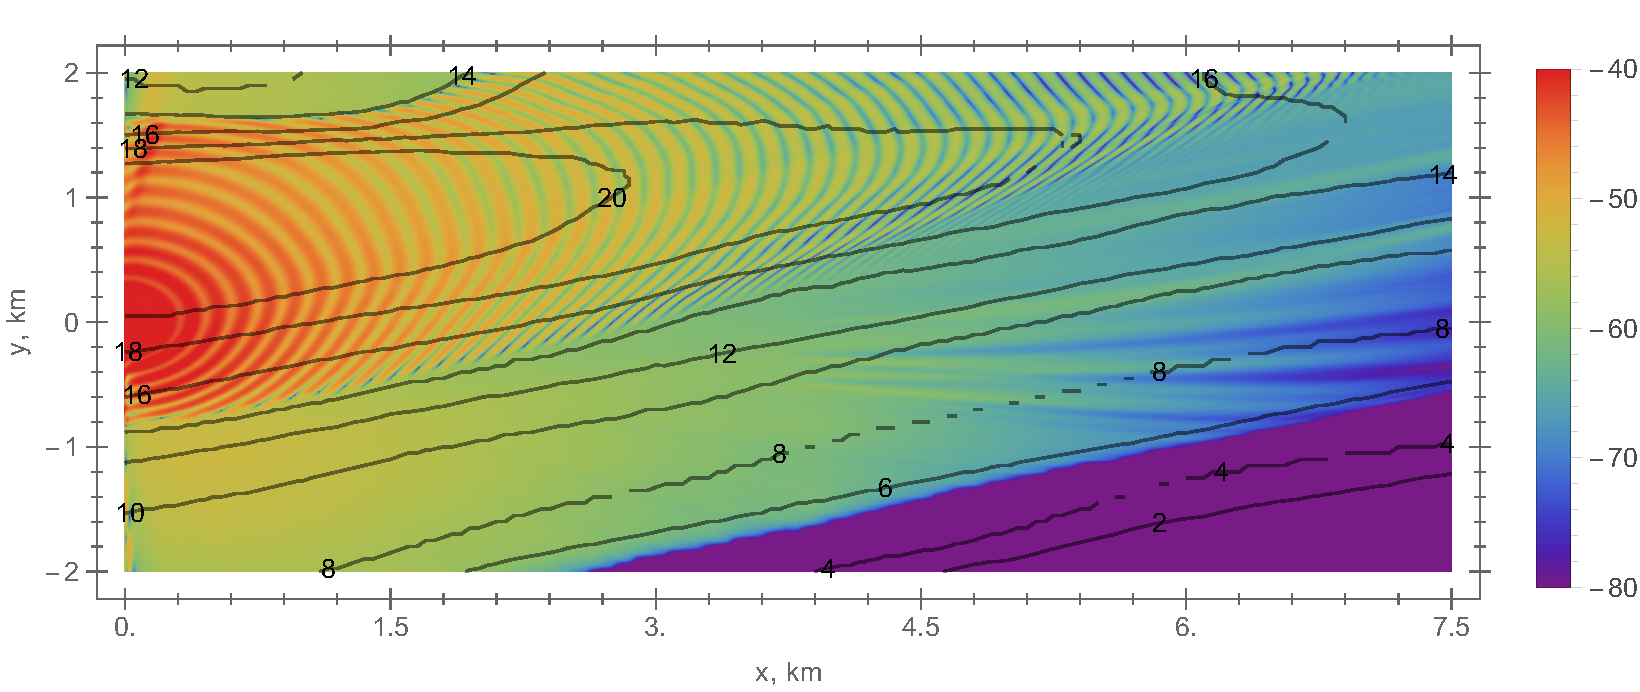
\includegraphics[width=\textwidth]{sakhalin_n11_z4.pdf}
                 \caption{SSP}
             \end{subfigure}
 		\end{figure}
 	\end{frame}

 	\note{Звуковое поле было вычислено на глубине $z=4\ \text{м.}$ Из рисунка видно, что решение ШМПУ существенно уступает решению, полученному методом SSP с большим порядком аппроксимации Падэ. Также можно заметить, как звук фокусируется в области с большей глубиной.}
    
     \begin{frame}{Программная реализация}
         \begin{block}{}
             \begin{itemize}
                 \item Язык C++17
                 \item Репозиторий: {\footnotesize \url{https://github.com/GoldFeniks/AMPLE}}
                 \item 70 коммитов, \textcolor{greenish}{++}12500, \textcolor{redish}{\textminus\textminus}7000
                 \item Зависимости
                 \begin{itemize}
                     \item Boost C++
                     \item ALGLIB
                     \item fftw3
                     \item nlohmann::json
                     \item Eigen
                 \end{itemize}
                 \item Модули
                 \begin{itemize}
                     \item CAMBALA\qquad {\footnotesize \url{https://github.com/Nauchnik/Acoustics-at-home/}}
                     \item DORK\qquad {\footnotesize \url{https://github.com/GoldFeniks/DORK}}
                     \item delaunay\qquad {\footnotesize \url{https://github.com/GoldFeniks/delaunay}}
                     \item zip\qquad {\footnotesize \url{https://github.com/GoldFeniks/zip}}
                 \end{itemize}
             \end{itemize}
         \end{block}
     \end{frame}
    
     \note{Для выполнения поставленных задач была написана программа на языке С++17. Репозиторий с кодом размешен на гитхабе.}

     \begin{frame}{Заключение}
         \begin{block}{Реализованы}
             \begin{itemize}
                 \item Трассировка лучей, соответствущих модам
                 \item Лучевые начальные условия
                 \item Расчёт решения, зависящего от $x,y,z$
                 \item SSP метод решения уравнения с использованием аппроксимации Падэ произвольного порядка
                 \item Вычисление импульса звукового сигнала и SEL
             \end{itemize}
         \end{block}
         \begin{block}{Возможные улучшения}
             \begin{itemize}
                 \item Использование пространственных неоднородностей параметров слоёв в воде и дне
                 \item Учёт межмодового взаимодействия
             \end{itemize}
         \end{block}
     \end{frame}

 	\note{Таким образом, в рамках проделанной работы были исследованы методы решения МПУ с использованием аппроксимации Падэ произвольного порядка, лучевых начальных условий и PML граничных условий, разработана численная схема их решения, разработан комплекс программ на языке C++, реализующий полученную численную схему с использованием пакета CAMBALA и возможностью вычисления временного ряда импульса звукового сигнала, значения распределения уровней SEL и координат распространения лучей, соответствующих вертикальным модам; проведены различные вычислительные эксперименты и изучена корректность и применимость полученного метода в сравнении с ШМПУ и другими методами решения уравнения Гельмгольца.}

     \begin{frame}
         \thispagestyle{empty}
         \addtocounter{framenumber}{-1}
         \ifPS
             \centerline{\Huge Спасибо за внимание}
         \fi
     \end{frame}

 	\note{Спасибо за внимание}
    
\end{document}